\documentclass[parskip=full]{scrartcl}
\usepackage[utf8]{inputenc}
\usepackage[T1]{fontenc}
\usepackage[ngerman]{babel}
\usepackage[hidelinks]{hyperref}
\usepackage{enumitem}
\usepackage{glossaries}
\usepackage{graphicx}

\usepackage[binary-units=true]{siunitx}
  \usepackage[autostyle=true,german=quotes]{csquotes}
\makeglossaries
%für die Nummerierung der Listen
\newcommand{\swtLabel}[1]{\textbf{/#1\arabic*0/}}
\newcommand{\testRef}[1]{[\ref{#1}]}
\newglossaryentry{PSE}{name=PSE,
                        description={Im PSE (Praxis der Softwareentwicklung)
                        lernen die Teilnehmer, ein vollständiges Softwareprojekt nach dem Stand der
                        Softwaretechnik in einem Team mit 5 bis 6 Teilnehmern
                        durchzuführen. Ziel ist es insbesondere, Verfahren des
                        Software-Entwurfs und der Qualitätssicherung praktisch
                        einzusetzen, Implementierungskompetenz umzusetzen, und
                        arbeitsteilig im Team zu kooperieren.}}
                      
\newglossaryentry{Lerngruppe}{name=Lerngruppe, plural=Lerngruppen,
description={Eine Lerngruppe ist ein Zusammenschluss von Studierenden, welche
gemeinsam eine Bewertung abgeben für die \glspl{Projekt}inteilung. Zusätzlich
werden sie bei der Einteilung gesondert berücksichtigt, sodass Studierende einer
Lerngruppe möglichst ein Team bilden oder als Gruppe einem Team angehören.
}}
\newglossaryentry{Guetekriterium}{name=Gütekriterium,
plural=Gütekriterien,description={Gütekriterien sind Kriterien, welche
die Güte einer Einteilung bestimmen. Anhand von Gütekriterien kann ein Vergleich
und eine Bewertung von Einteilungen vorgenommen werden. 
}}
\newglossaryentry{Projekt}{name=Projekt,
plural=Projekte, description={Ein Projekt ist ein zielgerichtetes Vorhaben,
welches von mindestens einem Team bearbeitet wird. Dieses Vorhaben wird von mehreren Projektbetreuern begleitet und unterstützt.
}}
\newglossaryentry{Projektbetreuer}{name=Projektbetreuer,
plural=Projektbetreuer, description={Ein Projektbetreuer ist eine Person, welche administrative und unterstützende Tätigkeiten eines oder mehrerer \glspl{Projekt} ausführt. Dabei kann ein Projektbetreuer mehrere Teams betreuen.
}}
\newglossaryentry{Admin}{name=Administrator,
plural=Administratoren, description={Ein Administrator ist eine Person, welche das \gls{PSE} administrativ unterstützt und das Produkt konfiguriert.
}}
\newglossaryentry{Studierender}{name=Studierender,
plural=Studierende, description={Ein Studierender ist eine Person, welche eingeschrieben ist an einer Universität. In diesem Kontext sind nur Studierende gemeint, welche sich für das \gls{PSE} angemeldet haben und an diesem teilnehmen wollen.
}}
\newglossaryentry{Team}{name=Team,
plural=Teams, description={Ein Team ist ein Zusammenschluss von Studierenden, welche gemeinsam ein Projekt bearbeiten.
}}
\newglossaryentry{SPO}{name=SPO,
plural=SPOs, description={Die SPO (Studienprüfungsordnung) regelt den Studienablauf, die Prüfungen und den Abschluss des Studiums.
}}
\newglossaryentry{Teilleistung}{name=Teilleistung, %bestandene weglassen?!
plural=bestandene Teilleistungen, description={Eine Teilleistung ist eine von den \glspl{Studierender}n zu erbringende Leistung, meist in Form einer schriftlichen Prüfung. Das bestehen einer oder mehrerer Teilleistungen führt zum bestehen eines \gls{Modul}s. Dies wird in der \gls{SPO} spezifiziert.
}}
\newglossaryentry{Modul}{name=Modul,
plural=Module, description={Ein Modul ist ein Zusammenschluss verschiedener Teilleistungen, welche das gleiche Thema abdecken. 
}}
\newglossaryentry{happyness}{name=Studierenden-Happyness,
plural=Studierenden-Happyness, description={Die Studierenden-Happyness ist ein
\gls{Guetekriterium} welches sich aus der  }} %TODO formulierung
\newglossaryentry{gesplitteteGruppe}{name=Anzahl der getrennten \glspl{Lerngruppe},
 description={ Die Anzahl der getrennten \glspl{Lerngruppe} ist ein
 \gls{Guetekriterium} welches angiebt, wieviele \glspl{Lerngruppe} bei der Einteilung
 auseinander gerissen wurden}}

\newglossaryentry{nichtZugeteilt}{name=Anzahl der nicht Zugeteilten,
 description={Die Anzahl der nicht Zugeteilten ist ein 
\gls{Guetekriterium} welches angiebt, wie viele Studierende bei einer einteilung
nicht zugeteilt wurden }}

\begin{document}

\title{\textbf{STRA\gls{PSE}}\\
        \large Supter Team Allocationt for \gls{PSE}}

\author{D. Biester, E. Dohse, P. Faller, P. Loth, L. Seufert, S. Kopmann}
        
\maketitle
 
\pagebreak
\tableofcontents
\pagebreak

\section{Zielbestimmung}

Die Einteilung zu den Projektgruppen für das Modul \gls{PSE} wurde
bisher über die Software \enquote{Webinscribe} gelöst.
\enquote{Webinscribe} ist dazu entworfen worden, Studierende zu Tutorien einzuteilen.
Zwar ähneln die Anforderungen an die \gls{PSE}-Teameinteilung denen, der Tutoriumseinteilung,
jedoch sind sie nicht absolut deckungsgleich. 
Dadurch ist die aktuelle Lösung mit Webinscribe umständlich in der Bedienung und lässt Wünsche bezüglich hilfreicher Features offen.
So müssen beispielsweise die angebotenen Themen als Tutorien eingetragen werden. 
Oder eine manuelle Änderung der Einteilung ist nicht über eine Eingabemaske möglich.

Dem tritt unser Produkt entgegen.
Da es speziell auf die Bedürfnisse der \gls{PSE}-Einteilung zugeschnitten ist, 
kann es eine konsistente und bequeme Benutzerschnittstelle anbieten.
Es löst das Problem, die Studierenden auf die angebotenen Projekte zu verteilen und kann dabei über die Eingabe von Parametern leicht konfiguriert werden.
Durch zusätzlich angebotene Features, wie die Verwaltung der Themen durch die Projektleiter selbst 
oder die Möglichkeit zur automatischen Benachrichtigung der betroffenen Studierenden und Betreuer über die
Einteilung, soll der Administrationsaufwand drastisch reduziert werden. 

Insgesamt entsteht dadurch für alle Beteiligten ein effektiver und smarter Workflow.


\subsection{Musskriterien}
 \begin{enumerate}[label=\swtLabel{M}]
   \item Datenerfassung: Studierende sollen auf einer Internetseite:   
   \begin{itemize}
     \item ihre Daten (siehe \ref{SDatenAnfang} bis \ref{SDatenEnde}),     
     \item ihre Projektvorlieben, 
     \item ihre bestandenen \glspl{Teilleistung},
     \item und gegebenenfalls ihre \glspl{Lerngruppe}
   \end{itemize}
   in das Produkt eingeben können.
   \item Studierende können sich mit ihrer Matrikelnummer und einem Passwort anmelden
   \item Der \gls{Admin} kann sich über einen Benutzernamen und ein Passwort authentifizieren
   \item Studierende können vor der Einteilung \glspl{Lerngruppe} erstellen, beitreten
    und diese wieder verlassen
    \item Übersicht über die eigene \gls{Lerngruppe} durch Studierende
    \item Vergabe von gemeinsamen \gls{Projekt}bewertungen für eine Lerngruppe
   \item Das Produkt teilt nach folgenden Kriterien Studierenden Teams zu:
   \label{Mzuteilung}
   \begin{itemize}
     \item Wer die Voraussetzungen nicht erfüllt wird nicht eingeteilt
     \item \glspl{Lerngruppe} sollten zusammenbleiben
     \item Präferenzen der Studierenden werden berücksichtigt
   \end{itemize}
     \item Konfiguration der Einteilungskriterien durch den \gls{Admin} möglich
   \item Manuelles Nachjustieren von berechneten Einteilungen durch den \gls{Admin} möglich
   \item Berechnung und Anzeige von \glspl{Guetekriterium}
   \item Im- und Export der Studierendendaten und
   Einteilungen als Datei zu Datensicherungszwecken
   \item Möglichkeit des sukzessiven Eintragens von \glspl{Projekt}n
   \item Verwalten mehrerer \glspl{SPO}
  
 \end{enumerate}


\subsection{Wunschkriterien}
Absteigend nach Priorität sortiert:
\begin{enumerate}[label=\swtLabel{W}]
  \item Möglichkeit zur Verwaltung der \glspl{Projekt} durch die Betreuer
      \item Nachjustierbarkeit bei Änderungen der SPO 
  
    \item Vergleich mehrerer Einteilungsergebnisse pro Semester unter verschiedenen Konfigurationen
  \item Stapelverarbeitung zur Berechnungen verschiedener Einteilungen mit
    unterschiedlichen Konfigurationen
  \item Abbrechen der Berechnung der Zuteilung möglich 
        \item Datenabgleich mit dem Campus Management System via \enquote{.csv}"=Datei %TODO Glossar CMS

    \item Wunschkriterien zur Lösung des Problems der Einteilung (\ref{Mzuteilung}):
    \begin{itemize}
        \item Eher 5er"=Teams als 6er"=Teams
        \item Teams möglichst mit Studierende im gleichen Fachsemester 
        \item Studierende bevorzugen, die bereits mehr Teilleistungen aus dem
        ersten Jahr bestanden haben.
        \item Wer sich zum zweiten mal bewirbt, soll bei der Einteilung bevorzugt werden
    \end{itemize}    
\item Anzeige der Projektdetails für Studierende
\item Warnung an den \gls{Admin}, falls er bei der manuellen Nachjustierung 
    der Einteilung die bei der Konfiguration angegebenen Grenzen überschreitet
    \item Authentifizierung via Shibboleth
    \item Verwaltung über mehrere Semester hinweg
    \item Verifikation der Studierenden-E-Mail-Adresse über einen
    Verifikationslink der an die, von Studierenden angegebenne E-Mail-Adresse
    geschickt wird
    \item Benachrichtigung der Studierenden und Mitarbeiter über die Einteilung   
    
    
    \item Mobile Version der Webseite zur Nutzung auf Smartphones und Tablets
    
    
    
\end{enumerate}

\subsection{Abgrenzungskriterien}
\begin{enumerate}[label=\swtLabel{AG}]
 
  \item Das Produkt ist nicht für die Nutzung außerhalb des KITs bestimmt %Please dont do the Deppenapostroph!

\item Die Einteilungsfunktion ist nur für die Einteilung zum \gls{PSE}, nicht
für die Vergabe sonstiger Praktikums- oder Tutoriumsplätze bestimmt
  
\end{enumerate}
\section{Produkteinsatz}
%Wissenschaftliche Mitarbeiter sollen durch das Produkt die Verwaltung der Pro-
%jekte und die Einteilung zur Praxis der Softwareentwicklung rechnerunterstützt
% durch-
%zuführen können.
%TODO formulierung
Das Produkt dient zum Einpflegen von \glspl{Projekt}n und zur Zuteilung von
Studierenden zu diesen \glspl{Projekt}n. Hierbei werden die Projektpräferenzen der
Studierenden berücksichtigt.


\subsection{Anwendungsbereiche}

\begin{itemize} 
  \item Projektverwaltung und "-zuteilung (universitärer Bereich) %TODO Detail
\end{itemize}

\subsection{Zielgruppe}
\begin{itemize} 
  \item \glspl{Studierender}
  \item \gls{Projektbetreuer}
  \item \gls{Admin}
\end{itemize}

\subsection{Betriebsbedingungen}
\begin{itemize} 
  \item Zugriff über eine Webseite
\end{itemize}
\section{Produktumgebung}

\begin{itemize} 
  \item Das Produkt läuft auf einem für alle Benutzer erreichbaren Webserver
\end{itemize}
\subsection{Server-Software}
\begin{itemize} 
  \item Webserver (\texttt{HTTP, SMTP})
  \item SQL"=Server
  \item ILP"=Solver Gurobi %TODO lizens
\end{itemize}
\subsection{Server-Hardware}
Mindestens:
\begin{itemize} 
  \item $\SI{16}{\giga\byte}$ Ram
  \item Intel i7 Quadcore mit 4 weiteren virtuellen Kernen 
  %TODO nachfragen was hier noch gebraucht wird
\end{itemize}
% hier überlegen ob man noch Orgware und Produkt-Schnittstellen dazu nimmt

\subsection{Client-Software}
\begin{itemize}
  \item Chome Version 54
  \item Firefox Version 50
\end{itemize}
oder neuer
\subsection{Client-Hardware}
\begin{itemize}
  \item Heim-PC mit Internetzugang %TODO wolllen wir igendeine art der  mobilen
  %nutzung zulassen? u
\end{itemize}
\section{Funktionale Anforderungen}

%\subsection{Funktionsübersicht}
%TODO Machen wir eine Fktübersicht?
\subsection{Studierendenfunktionen}

\subsubsection{Pflichtfunktionen}

\begin{enumerate}[label=\swtLabel{FA}]
  \item Registrierung eines Studierenden mit Datenerfassung: \testRef{UCstudReg}
  \label{FAregistrierung}
  \begin{itemize}
    \item Name, Matrikelnummer, E"=Mail"=Adresse, Semester
    \item Auswahl bestandener \glspl{Teilleistung} und der \gls{SPO}
    \item Auswahl noch ausstehender Nachprüfungen (vgl. \ref{SDatenAnfang} bis \ref{SDatenEnde})
  \end{itemize}
  \item Anmeldung mit Matrikelnummer und Passwort\label{FAStudanmeldung}
  \testRef{UCstudAnmeldung}
  \item Bewertung der \glspl{Projekt} \label{FAbewertung} \testRef{UCstudBewertung}
  \item Erstellung einer \gls{Lerngruppe} mit Name und Passwort
  \label{FAcreatelerng} \testRef{UCstudCrealernG}
  \item Bewertung der \glspl{Projekt} für die \gls{Lerngruppe} 
  \label{FAbewertung2} \testRef{UCstudBewertung}
  \item Beitritt zu einer \gls{Lerngruppe} \label{FAjoinLerng}
  \testRef{UCstudJoinLernG}
  \item Austritt aus einer \gls{Lerngruppe} \label{FAlergAustritt}
  \testRef{UCstudLeaveLernG}
  \item Übersicht der eigenen \gls{Lerngruppe} (Bewertung und Mitglieder)
  \label{FAcheckLerng} \testRef{UCstudUebersichtLernG}
  \item Abmeldung \label{FAStudabmeldung}
  \item Einsicht der Einteilungsergebnisse \label{FAStudeinsicht} \testRef{UCstudEinsichtEinteilung}
\end{enumerate}

\subsubsection{Wunschfunktionen}

\begin{enumerate}[label=\swtLabel{FA}, resume]
	\item Anzeigen von Projektbeschreibung in Bewertungseingabemaske
	\label{FAbeschreibung-Bewertung} \testRef{UCstudProjektbeschreibung}
	\item Anmeldung über u"=Account \label{FAstudUanmeldung} \testRef{UCstudAnmeldung}%TODO
	% Glossareintrag
	\item Verifikation der E"=Mail"= Adresse über einen Verifikationslink, der an
	die vom Studierenden angegebene E"=Mail"=Adresse versandt wird
	\label{FAemailverifikation} \testRef{UCstudVerifikationEmail}
	\item Anfordern eines neuen Passworts \label{FApasswortvergessen}
	\testRef{UCstudNewPasswort}
\end{enumerate}

\subsection{Betreuerfunktionen}
%TODO ein oder 2 Sätze in wieweit betreuer komplett wunsch ist 
\subsubsection{Wunschfunktionen}

\begin{enumerate}[label=\swtLabel{FA}, resume]
  \item Anmeldung  \label{FAbetreuerAnmeldung} \testRef{UCbetreuerAnmeldung}
  \item Erstellung eines \glspl{Projekt}s \label{FAbetreuerAddProjekt}
  \testRef{UCbetreuerThemaErstellenÄndern}
  \item Ändern der Projektdetails: Name, Beschreibung, Projektbetreuer,
        minimale und maximale Teilnehmerzahl, Anzahl der Teams
        \label{FAbetreuerChangeProjekt} \testRef{UCbetreuerThemaErstellenÄndern}%TODO Verweis auf
        % Produktdaten?
  \item Einsehen der Einteilung zu eigenen \glspl{Projekt}n
  \label{FAbetreuerEinsichtEinteilung}
  \testRef{UCbetreuerEinsichtEinteilungProjekt}
  \item Einsehen, welche zugeteilten \glspl{Studierender} noch Nachprüfungen
  ausstehen haben \label{FAbetreuerEinsichtNachpruefung}
  \item Einsehen, welche zugeteilten \glspl{Studierender} schon im Campus Management System für \gls{PSE} und TSE angemeldet sind 
  \label{FAbetreuerEinsichtTSE}
  \item Abmeldung \label{FAbetreuerAbmeldung}
  \item Noteneintragung für Studierende des betreuten \glspl{Projekt}s
  \label{FAbetreuerNoten} \testRef{UCbetreuerNoteneintragung}
  \item Einem \gls{Projekt} als Betreuer beitreten \label{FAbetreuerJoinProjekt}
  \testRef{UCbetreuerJoinProjekt}
  \item Ein \gls{Projekt} als Betreuer verlassen \label{FAbetreuerLeaveprojekt}
  \testRef{UCbetreuerLeaveProjekt}

\end{enumerate}

\subsection{Adminfunktionen}

\subsubsection{Pflichtfunktionen}

\begin{enumerate}[label=\swtLabel{FA}, resume]
  \item Anmeldung \label{FAadminAnmeldung}
  \item Initialisierung des Produktes bestehend aus einer Initialisierung der
  Datenbank und des Webservers
  % so?
  \label{FAadminInit} \testRef{UCadminInit}
  \item Setzten der frühest möglichen Anmeldezeit \label{FAadminAnmeldezeit}
  \testRef{UCadminAnmeldezeit}
  \item Setzen der Bewertungsdeadline \label{FAadminDeadline} \testRef{UCadminDeadline}
  \item Konfiguration der Einteilungsparameter \label{FAadminParameter}
  \testRef{UCadminEinteilungStart}
  %TODO Verweis auf GUI? oder Textuell? genauer was kann man konfiirerengu
  \item Starten der Einteilungsberechnung \label{FAadminEinteilungstart}
  \testRef{UCadminEinteilungStart}
  \item Übersicht über die aktuelle Einteilung \label{FAadminÜbersicht}
  \item Anzeige der \glspl{Guetekriterium} bestehend aus:
    \begin{itemize}
      \item \gls{happyness}
      \item \gls{nichtZugeteilt}
      \item \gls{gesplitteteGruppe}
    \end{itemize} \label{FAadminGüte}
  \item \glspl{Studierender} aus dem System entfernen \label{FAadminDeleteStudFromSystem}
  \item \glspl{Studierender} zum System hinzufügen \label{FAadminAddStudToSystem}
  \item \glspl{Studierender} zu einem \gls{Team} bei einer bereits berechneten
  Einteilung hinzufügen \label{FAadminAddStudToTeam}
  \item \glspl{Studierender} von einem \gls{Team} bei einer bereits berechneten
  Einteilung entfernen \label{FAadminRemoveStudFromTeam}
  \item \glspl{Studierender} zwischen \glspl{Team} bei einer bereits berechneten
  Einteilung verschieben  \label{FAadminMoveStudsBetweenTeams}
  \item Import einer Einteilung \label{FAimport}
  \item Export einer Einteilung \label{FAexport}
  \item Erstellung eines \glspl{Projekt}s \label{FAadminCreateProjekt}
  \testRef{UCadminProjektErstellenÄndern}
  \item Ändern der Projektdetails: Name, Beschreibung, Projektbetreuer, %TODO
        minimale und maximale Teilnehmerzahl, Anzahl der Teams
        \label{FAadminProjektänderung} \testRef{UCadminProjektErstellenÄndern}
  \item Löschen eines \glspl{Projekt}s \label{FAadminDeleteProjekt}
  \testRef{UCadminDeleteProjekt}
  \item Abmeldung \label{FAadminAbmeldung}
  \item Finale Wahl und Veröffentlichung der Einteilung \label{FAadminAuswahl}
  \testRef{UCadminEinteilungAuswahl}
\end{enumerate}

\subsubsection{Wunschfunktionen}

\begin{enumerate}[label=\swtLabel{FA}, resume]
  \item Abbrechen der Einteilungsberechnung \label{FAabbruch} \testRef{UCadminEinteilungStart}
  %TODO Was ist damit gemeint? \item Hinzufügen/Löschen von Studierenden
  %und Bearbeitung der Daten
  \item Hinzufügen von Berechnungen zur Stapelverarbeitung \label{FAadminStapel}
  \item Hinzufügen wählbarer Teilleistungen zu \glspl{SPO} \label{FAadminSPOhinzufügen}
  \item Entfernen wählbarer Teilleistungen zu \glspl{SPO} \label{FAadminSPOentfernen}
  \item \glspl{SPO} auswählen, die Studenten bei der Anmeldung angeben können
  \label{FAadminSPOAuswahl}
  \item Benachrichtigen der Studierenden und Projektbetreuer über die Einteilung
  per E"=Mail \label{FAadminBenachrichtigen} \testRef{UCadminEinteilungAuswahl}
  \item Erstellen von Betreueraccounts \label{FAadminCreateAccounts}
  \testRef{UCadminCreateBetreuer}
  %%TODO W70 und W100 Was genau soll man können?
  \item Import von \enquote{.csv}"=Dateien mit Informationen über bestandene
  \glspl{Teilleistung} der \glspl{Studierender}n aus dem Campus Management System 
  \label{FAimport2}
  \item Export von \enquote{.csv}"=Dateien mit Noten der \glspl{Studierender}n
  \label{FAexport2}
  \item Übersicht über bereits berechnete Einteilungen
  \label{FAadminUebersichtAlleEinteilungen} \testRef{UCadminEinteilungAuswahl}
  \item Warnung an den \gls{Admin}, falls er bei der manuellen Nachjustierung 
  der Einteilung die bei der Konfiguration angegebenen Grenzen überschreitet
  \label{FAadminWarnung}
\end{enumerate}

\subsection{Einteilungsfunktionen}
\subsubsection{Musskriterien}
\begin{enumerate}[label=\swtLabel{FA}, resume]
  \item Einteilen der Studierenden zu \glspl{Projekt}n. Hierbei werden folgende
  Kriterien, so weit möglich, berücksichtigt:
  \begin{itemize}
    \item Wer die, durch die \gls{SPO} gegebenen Voraussetzungen nicht erfüllt,
    wird nicht eingeteilt \label{FAeinteilung}
    \item Möglichst viele Studierende werden zu \glspl{Projekt}n zugeteilt 
    \item \glspl{Lerngruppe} bleiben zusammen
    \item Präferenzen der Studierenden werden berücksichtigt 
 \end{itemize} \label{FAeinteilungMussKriterien}
 \item Berechnung von \glspl{Guetekriterium} \label{FAguetekriterien}
\end{enumerate}

 \subsubsection{Wunschkriterien}
 
 \begin{enumerate}[label=\swtLabel{FA}, resume]
 \item Stapelverarbeitung von mehreren Einteilungen mit unterschiedlichen
 Konfigurationen \label{FAeinteilungStapel}\item Folgende Kriterien fließen in die Einteilung ein:
 \begin{itemize}
 	\item Wer sich zum zweiten mal bewirbt, soll bei der Einteilung bevorzugt werden
 	\item Eher 5er"=Teams als 6er"=Teams
 	\item Studierende in einem Team sind im gleichen Semester
 	\item Studierende höheren Semesters werden bevorzugt
 	\item Studierende, die bereits mehr Teilleistungen aus dem ersten Jahr
 	bestanden haben, werden bevorzugt
 \end{itemize} \label{FAeinteilungWunschKriterien}
\end{enumerate}

\section{Produktdaten}

\subsection{Administratordaten}
Über den \gls{Admin} werden folgende Daten gespeichert:
\begin{enumerate}[label=\swtLabel{D}] 
	\item Passwort
	\item Nutzername
\end{enumerate}

\subsection{Projektdaten} 
\subsection{Allgemeine Daten}
\begin{enumerate}[label=\swtLabel{D},resume]
  \item Aktuelles Semester
\end{enumerate}

Über ein Projekt sind folgende Daten zu speichern:
\begin{enumerate}[label=\swtLabel{D},resume] 
  \item Name
  \item Anzahl der Teams
  \item Beschreibung
  \item Projektbetreuer
  \item Minimale Teilnehmerzahl
  \item Maximale Teilnehmerzahl
  \item Internetadresse
\end{enumerate}

\subsection{Betreuerdaten}
Die zu einem Betreuer gehörenden Daten sind:
\begin{enumerate}[label=\swtLabel{D}, resume] 
	\item Name
	\item Vorname
	\item E"=Mail"=Adresse
	\item Passwort
\end{enumerate}
\subsection{Studierendendaten} 
Zu jedem Studierenden sollen folgende Daten gespeichert werden:
\begin{enumerate}[label=\swtLabel{D}, resume] 
  \item E"=Mail"=Adresse \label{SDatenAnfang}
  \item Name
  \item Vorname
  \item Im Falle von Authentifizierung ohne Shibboleth: Passwort
  \item Im Falle von Authentifizierung mit Shibboleth: u-Account
  \item Matrikelnummer
  \item Semester
  \item SPO
  \item bestandene \glspl{Teilleistung} 
  \item ausstehende Nachprüfungen \label{SDatenEnde}
  \item Falls keiner\gls{Lerngruppe} beigetreten: Bewertung, welchem Projekt er oder
  sie am liebsten zugeteilt würde
  \item Falls einer\gls{Lerngruppe} beigetreten: Die zugehörige\gls{Lerngruppe}
  
\end{enumerate}
\subsection{\glspl{Lerngruppe}daten} 
\begin{enumerate}[label=\swtLabel{D}, resume] 
  \item Name
  \item Passwort
  \item Bewertung der \glspl{Projekt}, zu welchem die \glspl{Lerngruppe}mitglieder
  (Studierende) am liebsten zugeteilt würden
  \item Mitglieder der\gls{Lerngruppe}
\end{enumerate}

\subsection{SPO-Daten}
\begin{enumerate}[label=\swtLabel{D}, resume]
	\item Name
	\item Notwendinge \glspl{Teilleistung}
	\item Wählbare \glspl{Teilleistung}
\end{enumerate}
\subsection{Semester"-Daten}
\begin{enumerate}[label=\swtLabel{D}, resume]
    \item Name
    \item Allgemeine Informationen zum \gls{PSE}
    \item Verfügbare \glspl{SPO}
    \item Startzeit der Studierendenanmeldung
    \item Deadline für Bewertungen
    \item bisherige Einteilungsergebnisse
\end{enumerate}

\section{Nichtfunktioale Anforderungen}

\begin{enumerate}[label=\swtLabel{NF}]
  \item Es müssen maximal 500 Studierende und 100 \glspl{Projekt} verwaltet werden
  können
  \item Für Studierende ist die Antwortzeit des Webservers im Schnitt nicht
  länger als 3 Sekunden. Ausgenommen hiervon sind \ref{FAregistrierung}, 
  \ref{FAbewertung} und \ref{FAbewertung2} bei welchen die Antwortzeit im
  Schnitt unter 10 Sekunden liegt
  \item Für den Administrator ist die Antwortzeit des Webservers im Schnitt nicht
  länger als 5 Sekunden. Ausgenommen hiervon sind \ref{FAadminInit}, \ref{FAimport},
  \ref{FAexport}, \ref{FAabbruch} und \ref{FAimport2} bei welchen die Antwortzeit im Schnitt
  unter 60 Sekunden liegt
  \item Für Betreuer ist die Antwortzeit des Webservers im Schnitt nicht
  länger als 5 Sekunden
  \item Die Einteilungsfunktion \ref{FAeinteilung} ist im Schnitt in unter 24
  Stunden fertig
	\item Der Session-Timeout der Internetseite liegt für Studierende bei 30
	Minuten
	\item Benutzbarkeit (Administrator): Nach Einführung von 4h können Nutzer die
	Einteilung administrieren
	\item Benutzbarkeit (Studierende): Mehr als 90\% der Studierenden können
	sich ohne Anleitung Registrieren, Anmelden und %TODO ab wann werden Studenten
	% bei der einteilung berücksichtigt diesen punkt dann hier einfügen
	\item Übertragbarkeit: %TODO
	\item Leichte Erweiterbarkeit der Einteilungsberechnung um weitere Kriterien
	
 
%TODO was fehlt hier noch

\end{enumerate}
\section{Globale Testfälle}
Folgende Funktionssequenzen sind zu überprüfen:

\begin{itemize}
  \item In der Studierendensicht:


\begin{enumerate} [label=\swtLabel{T}]
  
  
  \item Registrierung als Student, Erstellen oder beitreten einer\gls{Lerngruppe} und Abgeben einer Bewertung
  \item Deadlines zur Registrierung als Student und zur Bewertungsabgabe werden eingehalten
  

\end{enumerate}
  \item In der Adminsicht:
   \begin{enumerate} [label=\swtLabel{T}, resume]
  \item Einloggen als Administrator, Erstellung eines Semesters mit mehreren SPOs
  \item Einteilungsberechnung und anschließendem manuellen Editieren und
  Veröffentlichen dieser
\end{enumerate}
  \item In der Betreuersicht:
   \begin{enumerate} [label=\swtLabel{T}, resume]
  \item Einloggen als Projektbetreuer, Erstellung mehrerer Projekte
\end{enumerate}
  \item Bei den Einteilungsergebnissen
   \begin{enumerate} [label=\swtLabel{T}, resume]
  \item 
\end{enumerate}
\end{itemize}

\section{Systemmodelle}

\subsection{Szenarien}

\subsection{Anwendungsfälle}

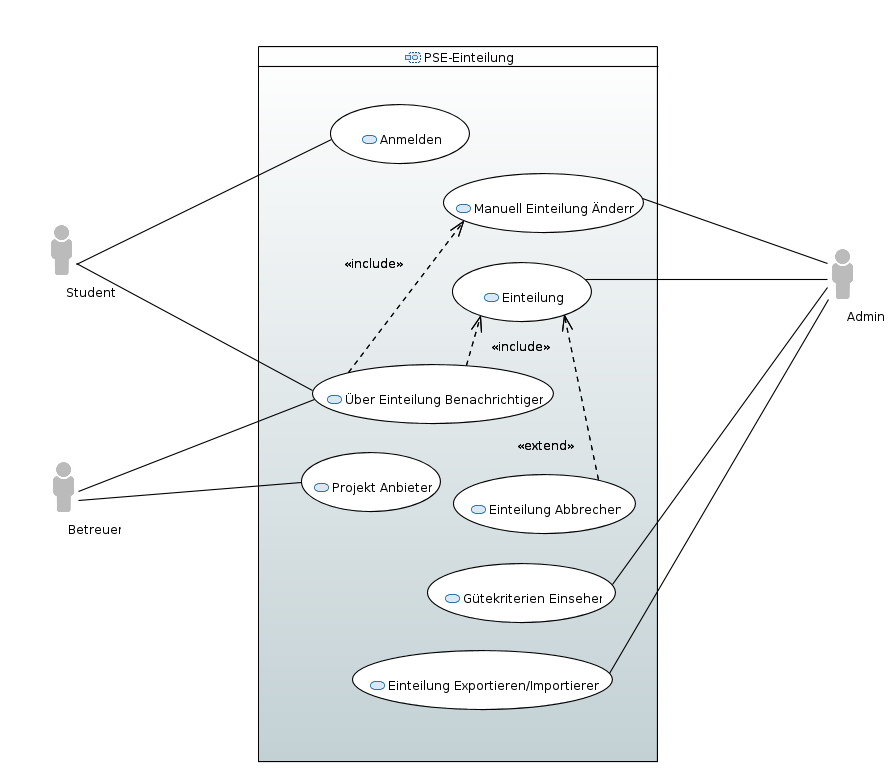
\includegraphics[width=\linewidth]{diagramme_pflichtenheft/UseCase_Diagram.PNG}
\captionof{figure}{Übersicht über die Anwendungsfälle}

\subsubsection{Studierende}

\begin{enumerate}[label=\swtLabel{S}]
	\item \label{UCstudReg}
    \begin{description}
  	\item[Anwendung:] Registrierung eines Studierenden
  	\item[Ziel:] Speichern der Studierendendaten in der Datenbank
  	\item[Vorbedingung:] Registrierung wurde freigeschaltet
  	\item[Nachbedingung(Erfolg):] Erfolgreiche Registrierung des Studierenden
  	\item[Nachbedingung(Fehlschlag):] Studierender ist weiterhin nicht
  	registriert
  	\item[Akteure:] Studierender
  	\item[Auslösen des Ereignisses:] Studierender will sich registrieren
  	\item[Beschreibung:]~
  	\begin{enumerate}
  	  \item[1.] Öffnen der Internetseite
      \item[2.] Klick auf Registrieren
      \item[3.] Ausfüllen der Registrierungsmaske %TODO Verweis auf Bild
      \item[4.] Abschicken der Daten
      \item[5.] Existiert der registrierte Account noch nicht, so wird der
      Studierende der Datenbank hinzugefügt
  	\end{enumerate}
  	\item[Erweiterungen:]~
  	\begin{enumerate}
  	  \item[zu 3)] Statt der Registrierungsmaske wird hier der u-Account
  	  verwendet
  	  \item[nach 4)] Dem Studierenden wird nach dem Abschicken seiner Daten eine
  	  \\
  	  Verifikations-Email gesendet. (siehe \testRef{UCstudVerifikationEmail})
  	 \end{enumerate} 
  	\item[Alternativen:]~
  	\begin{enumerate}
  	  \item[5a)] Wenn doch, so wird kein weiterer Eintrag hinzugefügt, sondern
  	  die zweite Registrierung abgebrochen
  	\end{enumerate} 
  	\item[benötigte FA:] \ref{FAregistrierung}, \ref{FAstudUanmeldung}
  \end{description}
%   
  
  \item \label{UCstudVerifikationEmail}
    \begin{description}
    \item[Anwendung:] Verifikation der E"=Mail"=Adresse
    \item[Ziel:] Verifikation der E"=Mail"=Adresse
    \item[Vorbedingung:] Studierender muss sich registriert haben und seine
    E"=Mail"=Adresse korrekt angegeben haben.
    \item[Nachbedingung(Erfolg):] Studierender kann sich nun Anmelden und hat
    Zugriff auf die Studierenden-Sicht
    \item[Nachbedingung(Fehlschlag):] Studierender kann sich nicht mit seinem
    Account anmelden
    \item[Akteure:] Studierender
    \item[Auslösen des Ereignisses:] Studierende registrieren sich und werden
    darauf hingewiesn ihre E"=Mail"=Adresse zu verifizieren.
    \item[Beschreibung:]~
    \begin{enumerate}
      \item[1.] E-mails über Drittsoftware abrufen.
      \item[2.] Klick auf den Verifikations-Link in der E"=Mail.      
    \end{enumerate}
    \item[Erweiterungen:] -keine-
    \item[Alternativen:] -keine-
    \item[benötigte FA:] \ref{FAemailverifikation}
      \end{description}
  
  \item \label{UCstudAnmeldung}
    \begin{description}
    \item[Anwendung:] Anmeldung eines Studierenden
    \item[Ziel:] Studierender wird angemeldet und kann seine Bewertungen ändern
  	\item[Vorbedingung:] Der Studierende hat sich vorher registriert
  	\item[Nachbedingung(Erfolg):] Der Studierende ist angemeldet
  	\item[Nachbedingung(Fehlschlag):] Der Studierende ist nicht angemeldet
  	\item[Akteure:] Studierender
  	\item[Auslösen des Ereignisses:] Studierender will sich anmelden
  	\item[Beschreibung:]~
  	\begin{enumerate}
  	  \item[1.] Studierender öffnet die Website
  	  \item[2.] Studierender füllt das Formular zum Anmelden aus und schickt
  	  dieses ab %TODO: Verweis auf Bild
  	  \item[3.] Sind die Anmeldedaten korrekt, so wird der Studierende zur
  	  Studierendensicht weitergeleitet
  	\end{enumerate}
  	\item[Erweiterungen:]
  	\begin{enumerate}
  	  \item[2)] Kein Formular, sondern Anmeldung über u-Account
  	\end{enumerate}    	
  	\item[Alternativen:]
	\begin{enumerate}
  	  \item[3a)] Wenn nicht, so erhält er eine Fehlermeldung
  	\end{enumerate}
  	\item[benötigte FA:] \ref{FAStudanmeldung}, \ref{FAstudUanmeldung}
  \end{description}
   
  
  \item \label{UCstudCrealernG}
  \begin{description}
  \item[Anwendung:] Studierender erstellt \gls{Lerngruppe}
  \item[Ziel:] Eine neue \gls{Lerngruppe} ist in der Datenbank vermerkt und der
  Ersteller ist erstes Mitglied dieser
  	\item[Vorbedingung:] Studierender ist angemeldet und befindet sich auf der
  	Website im Studierendenportal
  	\item[Nachbedingung(Erfolg):] Die \gls{Lerngruppe} wurde erfolgreich erstellt
  	\item[Nachbedingung(Fehlschlag):] Die \gls{Lerngruppe} wurde nicht erstellt
  	\item[Akteure:] Studierender
  	\item[Auslösen des Ereignisses:] Wille des Studierenden
  	\item[Beschreibung:]~
  	\begin{enumerate}
  	  \item[1.] Studierender gibt Name und Passwort in das Formular zum Erstellen
  	  einer \gls{Lerngruppe} ein und schickt dieses ab %TODO: Verweis einfügen
  	  \item[2.] Wenn noch keine \gls{Lerngruppe} mit diesem Namen existiert, so
  	  wird die \gls{Lerngruppe} in der Datenbank angelegt und der Ersteller wird
  	  erstes Mitglied
  	\end{enumerate}
  	\item[Erweiterungen:] -keine-
  	\item[Alternativen:] ~
  	\begin{enumerate}
  	  \item[2a)] Eine \gls{Lerngruppe} mit diesem Namen existiert schon. Dann
  	  wird keine weitere \gls{Lerngruppe} angelegt und dem Studierenden wird
  	  mitgeteilt, dass er den Namen der \gls{Lerngruppe} verändern soll
  	 \end{enumerate}
  	 \item[benötigte FA:] \ref{FAcreatelerng}
  \end{description}
   
  
  \item \label{UCstudJoinLernG}
  \begin{description}
  \item[Anwendung:] Studierender tritt \gls{Lerngruppe} bei
  \item[Ziel:] Studierender ist Mitglied einer \gls{Lerngruppe}
  	\item[Vorbedingung:] Studierender ist angemeldet und befindet sich auf der
  	Webseite in Studierendensicht
  	\item[Nachbedingung(Erfolg):] Der Studierende ist Mitglied der
  	\gls{Lerngruppe}
  	\item[Nachbedingung(Fehlschlag):] Der Studierende ist nicht Mitglied der
  	\gls{Lerngruppe}
  	\item[Akteure:] Studierender
  	\item[Auslösen des Ereignisses:] Der Studierende will einer \gls{Lerngruppe}
  	beitreten
  	\item[Beschreibung:]~
  	\begin{enumerate}
  	  \item[1.] Der Studierende gibt die Anmeldedaten der \gls{Lerngruppe} in das
  	  passende Formular ein und schickt dieses ab %TODO: Verweis
  	  \item[2.] Existiert die angegebene \gls{Lerngruppe}, so wird die
  	  Mitgliederliste derer um den Studierenden erweitert
  	\end{enumerate}
  	\item[Erweiterungen:]~
  	\begin{enumerate}
  	  \item[2a)] Ist die \gls{Lerngruppe} schon vollständig, so wird der
  	  Studierende nicht der Gruppe zugewiesen
  	  \item[3)] Ist der Studierende nicht der \gls{Lerngruppe} zugewiesen worden,
  	  so werden die zuletzt gespeicherten Bewertungen verwendet
  	  \item[4)] Der \glspl{Lerngruppe}ersteller wird per E-Mail informiert
  	 \end{enumerate}
  	\item[Alternativen:] ~
  	\begin{enumerate}
  	  \item[2a)] Existiert keine solche Gruppe, so schlägt der Beitritt fehl und
  	  der Studierende ist kein Mitglied der \gls{Lerngruppe}
  	 \end{enumerate}
  	 \item[benötigte FA:] \ref{FAjoinLerng}
  \end{description}
  
   \item \label{UCstudUebersichtLernG}
  \begin{description}
  \item[Anwendung:] Übersicht über \gls{Lerngruppe}
  \item[Ziel:] Studierender kann sehen wer in seiner \gls{Lerngruppe} ist
  	\item[Vorbedingung:] Studierender ist angemeldet und befindet sich auf der
  	Webseite in Studierendensicht. Weiterhin ist der Studierende Mitglied einer
  	\gls{Lerngruppe}
  	\item[Nachbedingung(Erfolg):] Studierender befindet sich nun in der
  	\glspl{Lerngruppe}übersicht
  	\item[Nachbedingung(Fehlschlag):] Der Studierende ist nicht in der
  	\glspl{Lerngruppe}übersicht
  	\item[Akteure:] Studierender
  	\item[Auslösen des Ereignisses:] Der Studierende möchte ansehen wer außer ihm
  	in der \gls{Lerngruppe} ist, in der er angemeldet ist
  	\item[Beschreibung:]~
  	\begin{enumerate}
  	  \item[1.] Der Studierende klickt auf \gls{Lerngruppe} %TODO Verweis
 
  	\end{enumerate}
  	\item[Erweiterungen:] -keine-
  	
  	\item[Alternativen:] -keine-
  	
  	 \item[benötigte FA:] \ref{FAcheckLerng}
  \end{description}
  
     \item \label{UCstudEinsichtEinteilung}
  \begin{description}
  \item[Anwendung:] Einsicht der Einteilungsergebnisse
  \item[Ziel:] \gls{Studierender} kann sehen welchem \gls{Projekt} er
  zugeteilt wurde
  	\item[Vorbedingung:] \gls{Studierender} ist angemeldet und befindet sich auf der
  	Webseite in Studierendensicht. 
  	\item[Nachbedingung(Erfolg):] \gls{Studierender} befindet sich in der Maske
  	Einteilungsergebnisse. %TODO verweis
  	Falls der \gls{Admin} die Einteilungsergebnisse bereits veröffentlicht hat,
  	kann er sehen, welchem \gls{Projekt} er zugeteilt wurde. Sonst sieht er, dass
  	die Einteilung noch im Gange ist %TODO Gehört der Abschnitt hier rein?
  	\item[Nachbedingung(Fehlschlag):] Der Studierende ist nicht in der
  	Maske Einteilungsergebnisse
  	\item[Akteure:] \gls{Studierender}
  	\item[Auslösen des Ereignisses:] Der Studierende möchte überprüfen, ob er
  	bereits einem Projekt zugeteilt wurde
  	\item[Beschreibung:]~
  	\begin{enumerate}
  	  \item[1.] Der Studierende klickt auf Einteilungsergebnisse
 
  	\end{enumerate}
  	\item[Erweiterungen:] -keine-

  	\item[Alternativen:] -keine-
  	
  	 \item[benötigte FA:] \ref{FAStudeinsicht}
  \end{description}
  
    \item \label{UCstudProjektbeschreibung}
  \begin{description}
  \item[Anwendung:] Anzeigen der Projektbeschreibung in Bewertungsmaske
  \item[Ziel:] Studierender kann sich während der Einteilung die Beschreibung
  der zu bewertenden Projekte nochmal ansehen
  	\item[Vorbedingung:] Studierender ist angemeldet und befindet sich in der
  	Projektbewertungsmaske %TODO verweis
  	
  	\item[Nachbedingung(Erfolg):] Studierender kann die Projektbeschreibung als
  	\enquote{Overlay} sehen %TODO wirklich als overlay? wie sieht der Studierend
  	%die beschreibunmg e
  	
  	\item[Nachbedingung(Fehlschlag):] Der Studierende kann die
  	Projektbeschreibung nicht sehen
  	\item[Akteure:] Studierender
  	\item[Auslösen des Ereignisses:] Der Studierende bewertet Projekte und möchte
  	sich über eines der \glspl{Projekt} genauer informieren
  	\item[Beschreibung:]~
  	\begin{enumerate}
  	  \item[1.] Der Studierende fährt mit seiner Maus über den Projektname 
 
  	\end{enumerate}
  	\item[Erweiterungen:] -keine-

  	\item[Alternativen:] -keine-

  	 \item[benötigte FA:] \ref{FAbeschreibung-Bewertung}
  \end{description}
  
      \item \label{UCstudLeaveLernG}
  \begin{description}
  \item[Anwendung:] Austritt aus einer \gls{Lerngruppe}
  \item[Ziel:] Studierender möchte aus einer \gls{Lerngruppe} austreten
  	\item[Vorbedingung:] Studierender ist angemeldet und befindet sich auf der
  	Webseite in Studierendensicht. Weiterhin ist er Mitglied
  	einer \gls{Lerngruppe}
  	%TODO verweis
  	
  	\item[Nachbedingung(Erfolg):] Studierender ist kein Mitglied der
  	\gls{Lerngruppe} mehr
  	
  	\item[Nachbedingung(Fehlschlag):] Studierender ist immernoch Mitglied der
  	\gls{Lerngruppe}
  	\item[Akteure:] Studierender
  	\item[Auslösen des Ereignisses:] Studierender möchte einer anderen
  	\gls{Lerngruppe} beitreten oder eigene Projektbewertungen abgeben
  	\item[Beschreibung:]~
  	\begin{enumerate}
  	  \item[1.] Der Studierende klickt auf \gls{Lerngruppe}. Nun befindet er sich
  	  in der \enquote{Lerngruppe}-Maske %TODO verweis
  	  \item[2.] Der Studierende klickt auf \enquote{Austreten}
 
  	\end{enumerate}
  	\item[Erweiterungen:] -keine-

  	\item[Alternativen:] -keine-

  	 \item[benötigte FA:] \ref{FAlergAustritt}
  \end{description}
%   
  
  \item \label{UCstudBewertung}
  \begin{description}
  \item[Anwendung:] Studierender bewertet \glspl{Projekt}
  \item[Ziel:] Der Studierende hat eine Bewertung abgegeben
  	\item[Vorbedingung:] Der Studierende ist angemeldet und im Studierendenportal der
  	Website
  	\item[Nachbedingung(Erfolg):] Die Bewertung wurde gespeichert
  	\item[Nachbedingung(Fehlschlag):] Die Bewertung wurde nicht gespeichert
  	\item[Akteure:] Studierender
  	\item[Auslösen des Ereignisses:] Des Studierendens Wille
  	\item[Beschreibung:]~
  	 \begin{enumerate}
  	   \item[1.] Der Studierende füllt die Bewertungsmaske aus %TODO: Verweis
  	   \item[2.] Der Studierende speichert die Bewertung ab
  	   \item[3.] Ist der Studierende Mitglied einer \gls{Lerngruppe}, so gilt die
  	   Bewertung gleichzeitig auch für alle anderen Mitglieder
  	 \end{enumerate}
  	\item[Erweiterungen:] -keine-
  	\item[Alternativen:] ~
  	\begin{enumerate}
  	  \item[3a)] Wenn nicht, so gilt sie nur für den Studierenden
  	 \end{enumerate}
  	\item[benötigte FA:] \ref{FAbewertung}, \ref{FAbewertung2}
  \end{description}
   
  
%  \item
%  \begin{description}
%  \item[Anwendung:] Studierender bewertet \glspl{Projekt} für
  % eine\gls{Lerngruppe}
%  \item[Ziel:] Die\gls{Lerngruppe} assoziiert mit dem Studierenden hat eine
  % Bewertung abgegeben
%  	\item[Vorbedingung:] Der Studierende ist als Leiter einer\gls{Lerngruppe}
  	% angemeldet und im Studierendenportal der Website
%  	\item[Nachbedingung(Erfolg):] Für die\gls{Lerngruppe} ist eine Bewertung
  	% eingetragen
%  	\item[Nachbedingung(Fehlschlag):] Für die\gls{Lerngruppe} ist keine (neue)
%  	Bewertung eingetragen
%  	\item[Akteure:] Studierender
%  	\item[Auslösen des Ereignisses:] Des Studierendens Wille
%  	\item[Beschreibung:]~
%  	 \begin{enumerate}
%  	   \item[1.] Der Studierende füllt die Bewertungsmaske aus
%  	   \item[2.] Der Studierende schließt die Bewertung ab
%  	 \end{enumerate}
%  	\item[Erweiterungen:] -keine-
%  	\item[Alternativen:] -keine-
%  	\item[benötigte FA:] \ref{FAbewertung2}
%  \end{description}
% TODO vermutlich löschen   
  
  \item \label{UCstudNewPasswort}
    \begin{description}
  	\item[Anwendung:] Passwort vergessen
  	\item[Ziel:] Erhalten eines neuen Passworts
  	\item[Vorbedingung:] Der Studierende hat schon einen Account
  	\item[Nachbedingung(Erfolg):] Der Studierende erhält eine E-Mail mit einem
  	neuen Passwort
  	\item[Nachbedingung(Fehlschlag):] Der Studierende erhält keine E-Mail
  	\item[Akteure:] Studierender
  	\item[Auslösen des Ereignisses:] Studierender hat sein Passwort vergessen
  	\item[Beschreibung:]~
  	\begin{enumerate}
  	  \item[1.] Öffnen der Internetseite
      \item[2.] Klick auf \enquote{Passwort vergessen}
      \item[3.] Eingabe der E"=Mail"=Adresse
      \item[4.] Der Studierende erhält eine E"=Mail mit seinem neuen Passwort
  	\end{enumerate}
  	\item[Erweiterungen:] -keine-
  	\item[Alternativen:] -keine-
  	\item[benötigte FA:] \ref{FApasswortvergessen}
  \end{description}
   
\end{enumerate}

\subsubsection{Betreuer}
\begin{enumerate} [label=\swtLabel{B}]
  \item \label{UCbetreuerAnmeldung}
	 \begin{description}
		\item[Anwendung:] Betreuer meldet sich an
  		\item[Ziel:] Anmeldung des Betreuers
  		\item[Vorbedingung:] Konto des Betreuers wurde angelegt
  		\item[Nachbedingung(Erfolg):] Betreuer ist angemeldet
  		\item[Nachbedingung(Fehlschlag):] Betreuer ist nicht angemeldet
  		\item[Akteure:] Betreuer
  		\item[Auslösen des Ereignisses:] Betreuer möchte sich anmelden
  		\item[Beschreibung]~
  		\begin{enumerate}
  			\item[1.] Der Betreuer gibt seine Zugangsdaten ein
  			\item[2.] Wenn die Anmeldedaten korrekt sind, wird er auf die
  			Betreueransicht weitergeleitet
  		\end{enumerate}
  		\item[Erweiterungen:] -keine-
  		\item[Alternativen:] ~
  		\begin{enumerate}
  		  \item[2a)] Wenn nicht, erhält er eine Fehlermeldung
  		\end{enumerate}  
  		\item[benötigte FA:] \ref{FAbetreuerAnmeldung}
  	\end{description}
   
  
  \item \label{UCbetreuerThemaErstellenÄndern}
	\begin{description}
  		\item[Anwendung:] Thema erstellen/ändern
  		\item[Ziel:] Eröffnung/Änderung eines \gls{PSE}-Themas
  		\item[Vorbedingung:] -keine-
  		\item[Nachbedingung(Erfolg):] Themendaten sind im System eingetragen
  		\item[Nachbedingung(Fehlschlag):] Themenfaten sind nicht im System
  		eingetragen
  		\item[Akteure:] Betreuer
  		\item[Auslösen des Ereignisses:] Betreuer möchte ein \gls{PSE}-Thema ins System
  		einfügen/ändern.
  		\item[Beschreibung:]~
  	\begin{enumerate}
  	  \item[1.] Betreuer befindet sich auf der Website mit den \gls{PSE}-Themen
  	  \item[2.] Existiert das Thema schon, so wählt der Betreuer dieses aus
  	  \item[3.] Betreuer füllt die Eingabemaske aus
  	  \item[4.] Betreuer speichert die neuen Daten ab
  	\end{enumerate}
  	\item[Erweiterungen:] -keine-
  	\item[Alternativen:]~
  	\begin{enumerate}
  	  \item[2a)] Wenn nicht, so fügt er ein neues hinzu
  	\end{enumerate}  
  	\item[benötigte FA:] \ref{FAbetreuerAddProjekt}, \ref{FAbetreuerChangeProjekt}
  \end{description}

 
  \item \label{UCbetreuerJoinProjekt}
	\begin{description}
  		\item[Anwendung:] Gruppenbetreuer werden
  		\item[Ziel:] Betreuer einer bestimmten Gruppe werden
  		\item[Vorbedingung:] Man ist noch nicht Betreuer der ausgewählten Gruppe
  		\item[Nachbedingung(Erfolg):] Erfolgreich Betreuer der ausgewählten
  		Gruppe geworden
  		\item[Nachbedingung(Fehlschlag):] Man ist nicht Betreuer der Gruppe
  		\item[Akteure:] Betreuer
  		\item[Auslösen des Ereignisses:] Betreuer möchte sich einer Gruppe
  		zuordnen
  		\item[Beschreibung:]~
  	\begin{enumerate} 
  	  \item[1.] Betreuer befindet sich auf der Website mit den \gls{PSE}-Gruppen
  	  \item[2.] Betreuer wählt die Gruppe aus, welcher er betreuen möchte
  	  \item[3.] Betreuer tritt der Gruppe bei
  	\end{enumerate}
  	\item[Erweiterungen:] -keine-
  	\item[Alternativen:] -keine-
  	\item[benötigte FA:] \ref{FAbetreuerJoinProjekt}
  \end{description}
  
  
  \item \label{UCbetreuerEinsichtEinteilungProjekt}
  \begin{description}
  	\item[Anwendung:] Einsicht der Einteilungsergebnisse
  	\item[Ziel:] Betreuer kann sehen, wer zu seinen Projekten zugeteilt wurde
  	\item[Vorbedingung:] \gls{Projektbetreuer} ist angemeldet und befindet sich auf der
  	Webseite in Betreuersicht  %TODO noch kein GUI entwurf
  	\item[Nachbedingung(Erfolg):] \gls{Projektbetreuer} befindet sich in der Maske
  	Einteilungsergebnisse. %TODO verweis
  	Falls der Admin die Einteilungsergebnisse bereits veröffentlicht hat, kann er
  	sehen, wer seinen \glspl{Projekt}n zugeteilt wurde. Sonst sieht er, dass die Einteilung
  	noch im Gange ist
  	\item[Nachbedingung(Fehlschlag):] Der \gls{Projektbetreuer} ist nicht in der
  	Maske Einteilungsergebnisse
  	\item[Akteure:] \gls{Projektbetreuer}
  	\item[Auslösen des Ereignisses:] Der \gls{Projektbetreuer} möchte wissen, wer zu seinen Projekt zugeteilt ist
  	\item[Beschreibung:]
  	\begin{enumerate}~
  		\item[1.] Der \gls{Projektbetreuer} klickt auf \enquote{Einteilungsergebnisse}  		
  	\end{enumerate}
  	\item[Erweiterungen:] -keine-
  	
  	\item[Alternativen:] -keine-
  	
  	\item[benötigte FA:] \ref{FAbetreuerEinsichtEinteilung}
  \end{description}
   
  
  \item \label{UCbetreuerLeaveProjekt}
	\begin{description}
  		\item[Anwendung:] Gruppe verlassen
  		\item[Ziel:] Eine Gruppe nicht mehr betreuen
  		\item[Vorbedingung:] Man ist Betreuer einer Gruppe, in der noch mindestens
  		ein anderer Betreuer ist.
  		\item[Nachbedingung(Erfolg):] Man betreut die Gruppe nicht länger.
  		\item[Nachbedingung(Fehlschlag):] Man ist immernoch Betreuer der Gruppe.
  		\item[Akteure:] Betreuer
  		\item[Auslösen des Ereignisses:] Betreuer möchte aus Gruppe austreten.
  		\item[Beschreibung:]~
  	\begin{enumerate} 
  	  \item[1.] Betreuer befindet sich auf der Website mit den \gls{PSE}-Gruppen, die
  	  er betreut.
  	  \item[2.] Betreuer wählt die Gruppe aus, welche er verlassen möchte.
  	  \item[3.] Betreuer verlässt die Gruppe.
  	\end{enumerate}
  	\item[Erweiterungen:] -keine-
  	\item[Alternativen:] -keine-
  	\item[benötigte FA:] \ref{FAbetreuerLeaveprojekt}
  \end{description}
   
  
  \item \label{UCbetreuerNoteneintragung}
    \begin{description}
  	\item[Anwendung:] Noten für Gruppenteilnehmer eintragen
  	\item[Ziel:] Speichern der Noten in der Datenbank
  	\item[Vorbedingung:] Gruppe hat Studierenden als Teilnehmer
  	\item[Nachbedingung(Erfolg):] Eintragung/Änderung der Noten
  	\item[Nachbedingung(Fehlschlag):] Notenänderung wird verworfen
  	\item[Akteure:] Betreuer
  	\item[Auslösen des Ereignisses:] Betreuer möchte Noten eintragen
  	\item[Beschreibung:]~
  	\begin{enumerate} 
  	  \item[1.] Betreuer befindet sich auf der Website mit der Notenübersicht
  	  \item[2.] Betreuer trägt neue Noten für eine beliebige Phase ein oder
  	  ändert bestehende Noten
  	\end{enumerate}
  	\item[Erweiterungen:] -keine-
  	\item[Alternativen] -keine-
  	\item[benötigte FA:] \ref{FAbetreuerNoten}
  \end{description}
   
\end{enumerate}


\subsubsection{Administrator}
\begin{enumerate} [label=\swtLabel{A}]
	
	\item \label{UCadminInit}
	\begin{description}
		\item[Anwendung:] Initialisierung des Produktes
		\item[Ziel:] Das Produkt soll für den Einsatz vorbereitet werden
		\item[Vorbedingung:] -keine-
		\item[Nachbedingung(Erfolg):] Das Produkt ist einsatzbereit und kann über das Webinterface bedient werden
		\item[Nachbedingung(Fehlschlag):] Das Produkt ist nicht einsatzbereit und gibt
		eine aussagekräftige Fehlermeldung aus
		\item[Akteure:] \gls{Admin}
		\item[Auslösen des Ereignisses:] Beginn des \gls{PSE}
		\item[Beschreibung:]
		\begin{enumerate} [label=\arabic*.]~
			\item Der \gls{Admin} stellt auf dem Server Gurobi bereit %TODO Gurobi Glossar
			\item Er startet Web"= und Datenbankserver 
			\item Er startet das Produkt
		\end{enumerate}
		\item[Erweiterungen:] -keine-
		\item[Alternativen:]~
		\begin{enumerate}
			\item[2 a)] Kann entfallen, wenn Server bereits in Betrieb sind
		\end{enumerate}
		\item[benötigte FA:] \ref{FAadminInit}
	\end{description}
	
	\item \label{UCadminAnmeldezeit}
	\begin{description}
		\item[Anwendung:] Setzten der frühesten möglichen Anmeldezeit
		\item[Ziel:] Ein frühestmöglicher Zeitpunkt für die Anmeldung von \glspl{Studierender}n soll festgelegt werden
		\item[Vorbedingung:] \gls{Admin} ist angemeldet und in der Adminansicht der Website
		\item[Nachbedingung(Erfolg):] Vor dem eingegeben Datum können sich
		\glspl{Studierender} nicht mehr anmelden und einloggen
		\item[Nachbedingung(Fehlschlag):] Anmelden und Einloggen sind weiter möglich
		\item[Akteure:] \gls{Admin}
		\item[Auslösen des Ereignisses:] Beginn des \gls{PSE}
		\item[Beschreibung:]~
		\begin{enumerate}[label=\arabic*.]
			\item Der \gls{Admin} klickt auf den Reiter \enquote{Einstellungen}
			\item Er trägt in das Feld \enquote{Startzeit der Studierendenanmeldung} ein Datum und eine Uhrzeit ein
		\end{enumerate}
		\item[Erweiterungen:] -keine-
		\item[Alternativen:] -keine-
		\item[benötigte FA:] \ref{FAadminAnmeldezeit}
	\end{description}	
	
	\item \label{UCadminDeadline}
	\begin{description}
		\item[Anwendung:] Setzten der Bewertungsdeadline
		\item[Ziel:] Ein spätester Zeitpunkt für die Anmeldung von \glspl{Studierender}n soll festgelegt werden
		\item[Vorbedingung:] \gls{Admin} ist angemeldet und in der Adminansicht der Website
		\item[Nachbedingung(Erfolg):] Nach dem eingegeben Datum können sich keine
		\glspl{Studierender}n mehr anmelden
		\item[Nachbedingung(Fehlschlag):] Anmelden ist weiter möglich
		\item[Akteure:] \gls{Admin}
		\item[Auslösen des Ereignisses:] Beginn des \gls{PSE}
		\item[Beschreibung:]~
		\begin{enumerate}[label=\arabic*.]
			\item Der \gls{Admin} klickt auf den Reiter \enquote{Einstellungen}
			\item Er trägt in das Feld \enquote{Deadline für Studierendenbewertung} ein Datum und eine Uhrzeit ein
		\end{enumerate}
		\item[Erweiterungen:] -keine-
		\item[Alternativen:] -keine-
		\item[benötigte FA:] \ref{FAadminDeadline}
	\end{description}
	
  \item \label{UCadminProjektErstellenÄndern}
    \begin{description}
  	\item[Anwendung:] Hinzufügen/Ändern eines Projekts
  	\item[Ziel:] Einfügen/Änderung von Projektdaten in der Datenbank
  	\item[Vorbedingung:] -keine-
  	\item[Nachbedingung(Erfolg):] Neue Projektdaten sind eingetragen
  	\item[Nachbedingung(Fehlschlag):] Neue Projektdaten sind nicht eingetragen
  	\item[Akteure:] Administrator, Institut
  	\item[Auslösen des Ereignisses:] Administrator bekommt Projektdaten von einem
  	Institut vorgelegt
  	\item[Beschreibung:]~
  	\begin{enumerate} 
  	  \item[1.] Projektübersicht öffnen
  	  \item[2.] Wenn das Projekt schon existiert, so werden die Projektdaten
  	  verglichen
  	  \item[3.] Stimmen die Projektdaten nicht überein, so werden die betroffenen
  	  Daten angepasst
  	  \item[4.] Durch Abspeichern der Eingaben werden die Daten in der Datenbank
  	  angepasst
  	\end{enumerate}
  	\item[Erweiterungen:] -keine-
  	\item[Alternativen:]~
  	\begin{enumerate}
  	  \item[2a)] Wenn nicht, dann wird das Projekt neu angelegt
  	  \item[3a)] Falls doch, so ist dieser Anwendungsfall abgeschlossen
  	\end{enumerate} 
  	\item[benötigte FA:] \ref{FAadminCreateProjekt}, \ref{FAadminProjektänderung}
  \end{description}
   
  
  \item \label{UCadminDeleteProjekt}
  \begin{description}
  \item[Anwendung:] Löschen eines Projektes
  \item[Ziel:] Löschen eines Projektes aus der Datenbank
  	\item[Vorbedingung:] Projekt existiert bereits in der Datenbank und die
  	Studierenden konnten noch keine Bewertungen abgeben
  	\item[Nachbedingung(Erfolg):] Projekt ist aus der Datenbank entfernt
  	\item[Nachbedingung(Fehlschlag):] Projekt ist immer noch in der Datenbank
  	\item[Akteure:] Administrator, Institut %TODO Institut kommt hier zum ersten mal vor
  	\item[Auslösen des Ereignisses:] Institut zieht ein Projekt zurück oder es
  	fehlen Daten bei Beginn der Einteilung
  	\item[Beschreibung:]~
  	\begin{enumerate} 
  	  \item[1.] Projektübersicht öffnen
  	  \item[2.] Projekt aus Liste entfernen
  	  \item[3.] Projektdaten werden aus der Datenbank entfernt
  	\end{enumerate}
  	\item[Erweiterungen:] -keine-
  	\item[Alternativen:] -keine-
  	\item[benötigte FA:] \ref{FAadminDeleteProjekt}
  \end{description}
   
  
  \item \label{UCadminEinteilungStart}
  \begin{description}
  \item[Anwendung:] Teameinteilung
  \item[Ziel:] Finden einer Teameinteilung nach ausgewählten Parametern
  	\item[Vorbedingung:] Alle \glspl{Projekt} in der Datenbank sind vollständig
  	\item[Nachbedingung(Erfolg):] Es wurde eine Teameinteilung gefunden
  	\item[Nachbedingung(Fehlschlag):] Es wurde keine Teameinteilung gefunden
  	\item[Akteure:] Administrator
  	\item[Auslösen des Ereignisses:] Entscheidung des Administrators bzw.
  	zeitliche Deadline
  	\item[Beschreibung:]~
  	\begin{enumerate} 
  	  \item[1.] Einstellen der Parameter nach denen eingeteilt werden soll
  	  \item[2.] Starten der Berechnung über Schaltfläche
  	  \item[3.] Sind alle \glspl{Projekt} vollständig angegeben, so startet die
  	  Berechnung
  	  \item[4.] Nach Abschluss der Berechnung wird das Ergebnis inklusive
  	  eingestellter Parameter abgespeichert
  	\end{enumerate}
  	\item[Erweiterungen:] -keine-
  	\item[Alternativen:] ~
  	\begin{enumerate}
  	  \item[3a)] Wenn nicht, so startet die Berechnung nicht und der Fall ist
  	  beendet
  	  \item[4a)] Hier ist auch ein frühzeitiger Abbruch durch den Administrator
  	  möglich. Dies wird im Ergebnis vermerkt.
  	 \end{enumerate}  
  	 \item[benötigte FA:] \ref{FAadminParameter},
  	 \ref{FAadminEinteilungstart}, \ref{FAabbruch}
  \end{description}
   
  
  \item \label{UCadminEinteilungAuswahl}
  \begin{description}
  \item[Anwendung:] Finale Auswahl der Einteilung
  \item[Ziel:] Finden der bestmöglichen Teameinteilung
  	\item[Vorbedingung:] Es wurde mindestens eine Berechnung durchgeführt
  	\item[Nachbedingung(Erfolg):] Es wurde eine Teameinteilung ausgewählt
  	\item[Nachbedingung(Fehlschlag):] Es wurde keine Teameinteilung ausgewählt
  	\item[Akteure:] Administrator
  	\item[Auslösen des Ereignisses:] Entscheidung des Administrators bzw.
  	zeitliche Deadline
  	\item[Beschreibung:]~
  	\begin{enumerate} 
  	  \item[1.] Der Administrator wählt eine der berechneten Einteilung final aus
  	  \item[2.] Wurde ein Studierender zugewiesen, so wird seinem
  	  Datenbankeintrag sein Team hinzugefügt
  	\end{enumerate}
  	\item[Erweiterungen:]~
  	\begin{enumerate}
  	  \item[nach 2)] Betreuer werden über ihre Teams informiert
  	  \item[nach 2)] Die Studierenden werden über ihre Einteilung informiert
  	 \end{enumerate}
  	\item[Alternativen:] ~
  	\begin{enumerate}
  	  \item[2a)] Wird ein Studierender nicht zugewiesen, so wird dies ebenfalls
  	  in der Datenbank vermerkt
  	 \end{enumerate}  
  	 \item[benötigte FA:] \ref{FAadminAuswahl},
  	 \ref{FAadminBenachrichtigen}, \ref{FAadminUebersichtAlleEinteilungen} 
  \end{description}
   
  
%  \item \label{UCadminInit}
%  \begin{description}
%  \item[Anwendung:] Einteilung eines Studierenden
%  \item[Ziel:] Manuelle Einteilung eines Studierenden
%  	\item[Vorbedingung:] Automatische Teameinteilung ist abgeschlossen
%  	\item[Nachbedingung(Erfolg):] Der Studierende wurde hinzugefügt
%  	\item[Nachbedingung(Fehlschlag):] Der Studierende wurde nicht hinzugefügt
%  	\item[Akteure:] Administrator, Studierender
%  	\item[Auslösen des Ereignisses:] Studierender meldet sich beim Administrator
%  	\item[Beschreibung:]~
%  	 \begin{enumerate} 
%  	   \item[1.] Wenn sich der Studierende noch nicht im System befindet
%  	   überprüft der Administrator, ob die Anforderungen für das \gls{PSE}
  	   % erfüllt sind
%  	   \item[2.] Hat der Studierende die Anforderungen erfüllt, so versucht der
%  	   Administrator ihn einem Team zuzuteilen
%  	   \item[3.] Hat der Administrator ein Team gefunden so fügt er den
%  	   Studierenden über eine Eingabemaske dem System hinzu
%  	 \end{enumerate}
%  	\item[Erweiterungen:]~
%  	 \begin{enumerate}
%  	   \item [nach 3)] Betreuer, sowie andere Mitglieder des Projekts, werden
%  	   über das neue Mitglied per E-Mail informiert 
%  	 \end{enumerate}  
%  	\item[Alternativen:] ~
%  	 \begin{enumerate}
%  	  \item[1a)] Falls doch, so wurde er schon vorher abgelehnt/nicht zugewiesen
%  	  und wird nicht eingeteilt. Dieser Fall ist damit abgeschlossen
%  	  \item [2a)] Falls er die Anforderungen nicht erfüllt, so wird er auch
  	  % nicht zugeteilt und dieser Fall ist abgeschlossen
%  	 \end{enumerate}  
%  	 \item[benötigte FA:] \ref{FAadminDeleteStudFromSystem}
%  \end{description} 
% TODO Umformulieren, sodass er zu einem der Punkte passt, oder löschen
     
  \item \label{UCadminCreateBetreuer}
  \begin{description}
  \item[Anwendung:] Erstellen eines Betreueraccounts
  \item[Ziel:] Hinzufügen eines Betreuers in das System
  	\item[Vorbedingung:] -keine-
  	\item[Nachbedingung(Erfolg):] Der Betreueraccount wurde erstellt
  	\item[Nachbedingung(Fehlschlag):] Der Betreueraccount wurde nicht erstellt
  	\item[Akteure:] Administrator
  	\item[Auslösen des Ereignisses:] Betreuer benötigt Account
  	\item[Beschreibung:]~
  	 \begin{enumerate} 
  	   \item[1.] Der Administrator öffnet die Maske zum Erstellen eines
  	   Betreueraccounts  
  	   \item[2.] Der Administrator füllt die Maske aus und schickt sie ausgefüllt
  	   ab
  	   \item[3.] Wenn noch kein Account mit dem angegebenen Namen existiert, so
  	   wird der neue Account der Datenbank hinzugefügt
  	 \end{enumerate} 
  	\item[Erweiterungen:]~
  	 \begin{enumerate}
  	   \item[4)] Der Betreuer erhält seine Zugangsdaten per E-Mail
  	 \end{enumerate}  
  	\item[Alternativen:] ~
  	 \begin{enumerate}
  	  \item[3a)] Falls doch, so wird eine Fehlermeldung angezeigt
  	 \end{enumerate}  
  	 \item[benötigte FA:] \ref{FAadminCreateAccounts}
  \end{description}
  
\end{enumerate}  
\subsection{Objektmodelle}

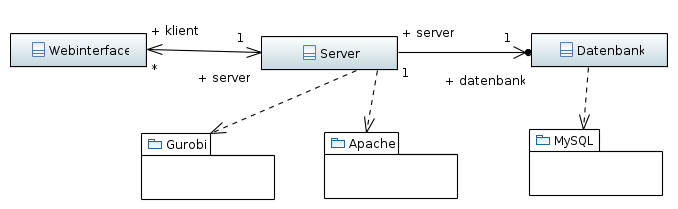
\includegraphics[width=\linewidth]{diagramme_pflichtenheft/ClassDiagram.PNG}
\captionof{figure}{Schematischer Aufbau des Produkts}

%TODO Brauchen wir das? \subsection{Dynamische Modelle}

\subsection{Benutzerschnittstelle}
\begin{enumerate}
  \item Es ist eine Benutzung rein über ein Web-Interface vorgesehen
  \item Es sind drei Sichten zu unterscheiden:
        \begin{itemize}
          \item die Sicht des Studierenden
          \item die Sicht des Betreuers
          \item die Sicht des Administrators
        \end{itemize}
  \item Die jeweiligen sichten sind erst nach der Anmeldung einzusehen 
  \item Studierende dürfen nur auf ihre eigenen Daten und falls sie in einer
 \gls{Lerngruppe} sind auf die Daten dieser zugreifen 
\subsubsection{GUI}
{\centering
\fbox{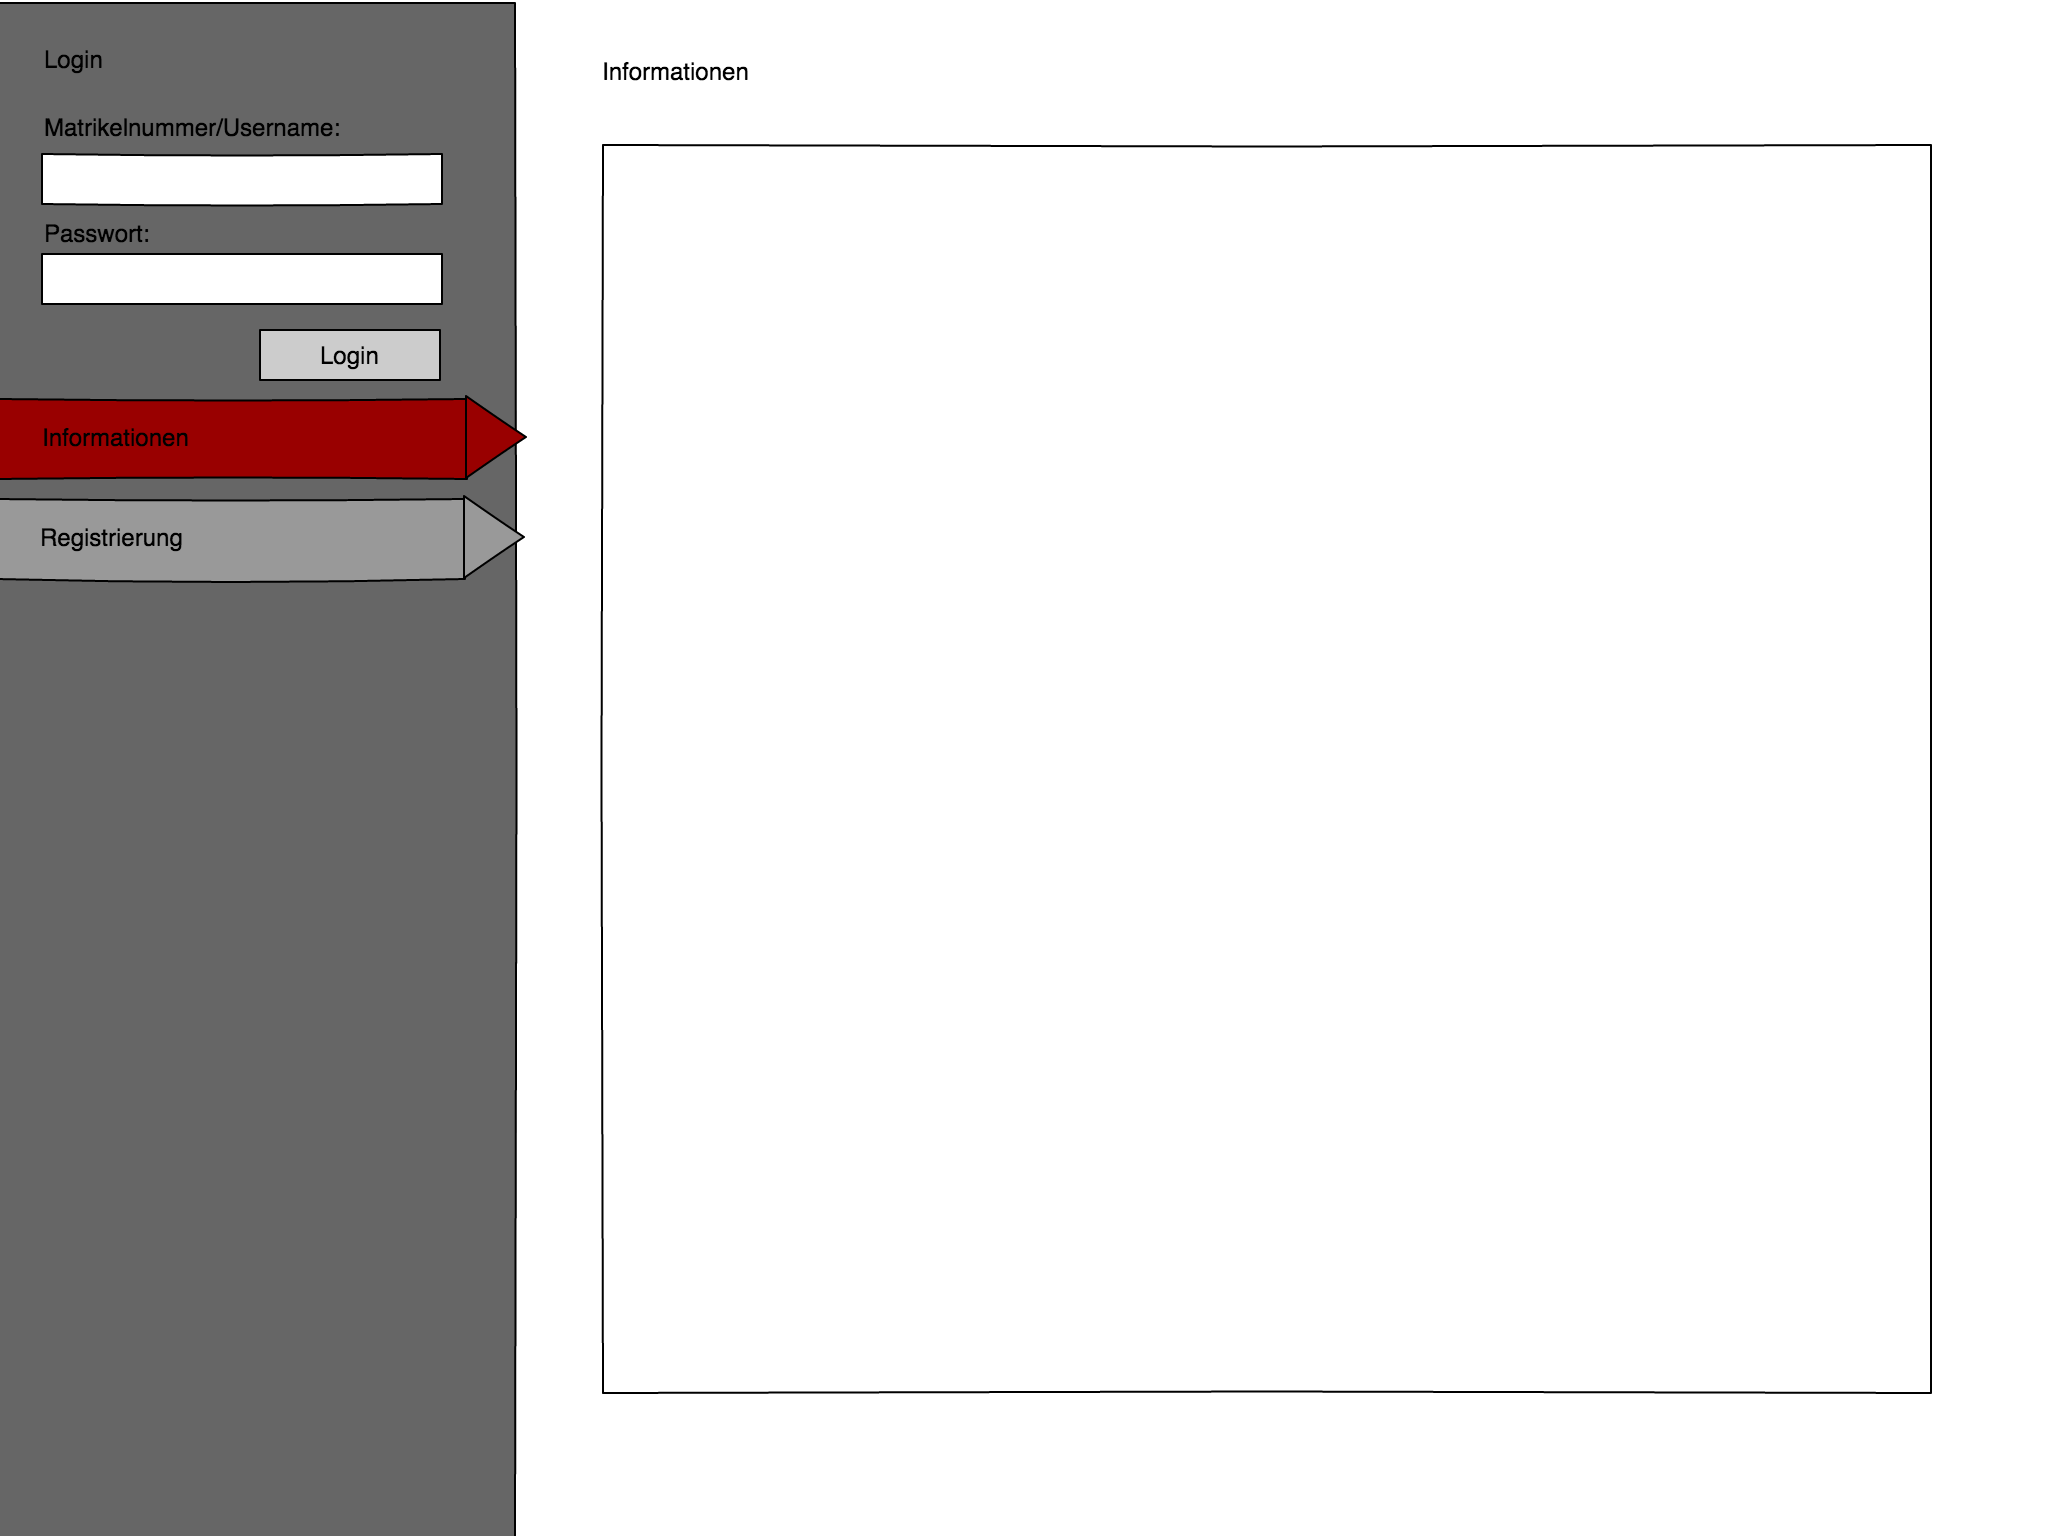
\includegraphics[width=\textwidth,
keepaspectratio=true]{gui/index.png}}
\captionof{figure}{Startseite} \label{GUIindex}


\setlength{\textheight}{297mm}
\setlength{\headheight}{0mm}
\fbox{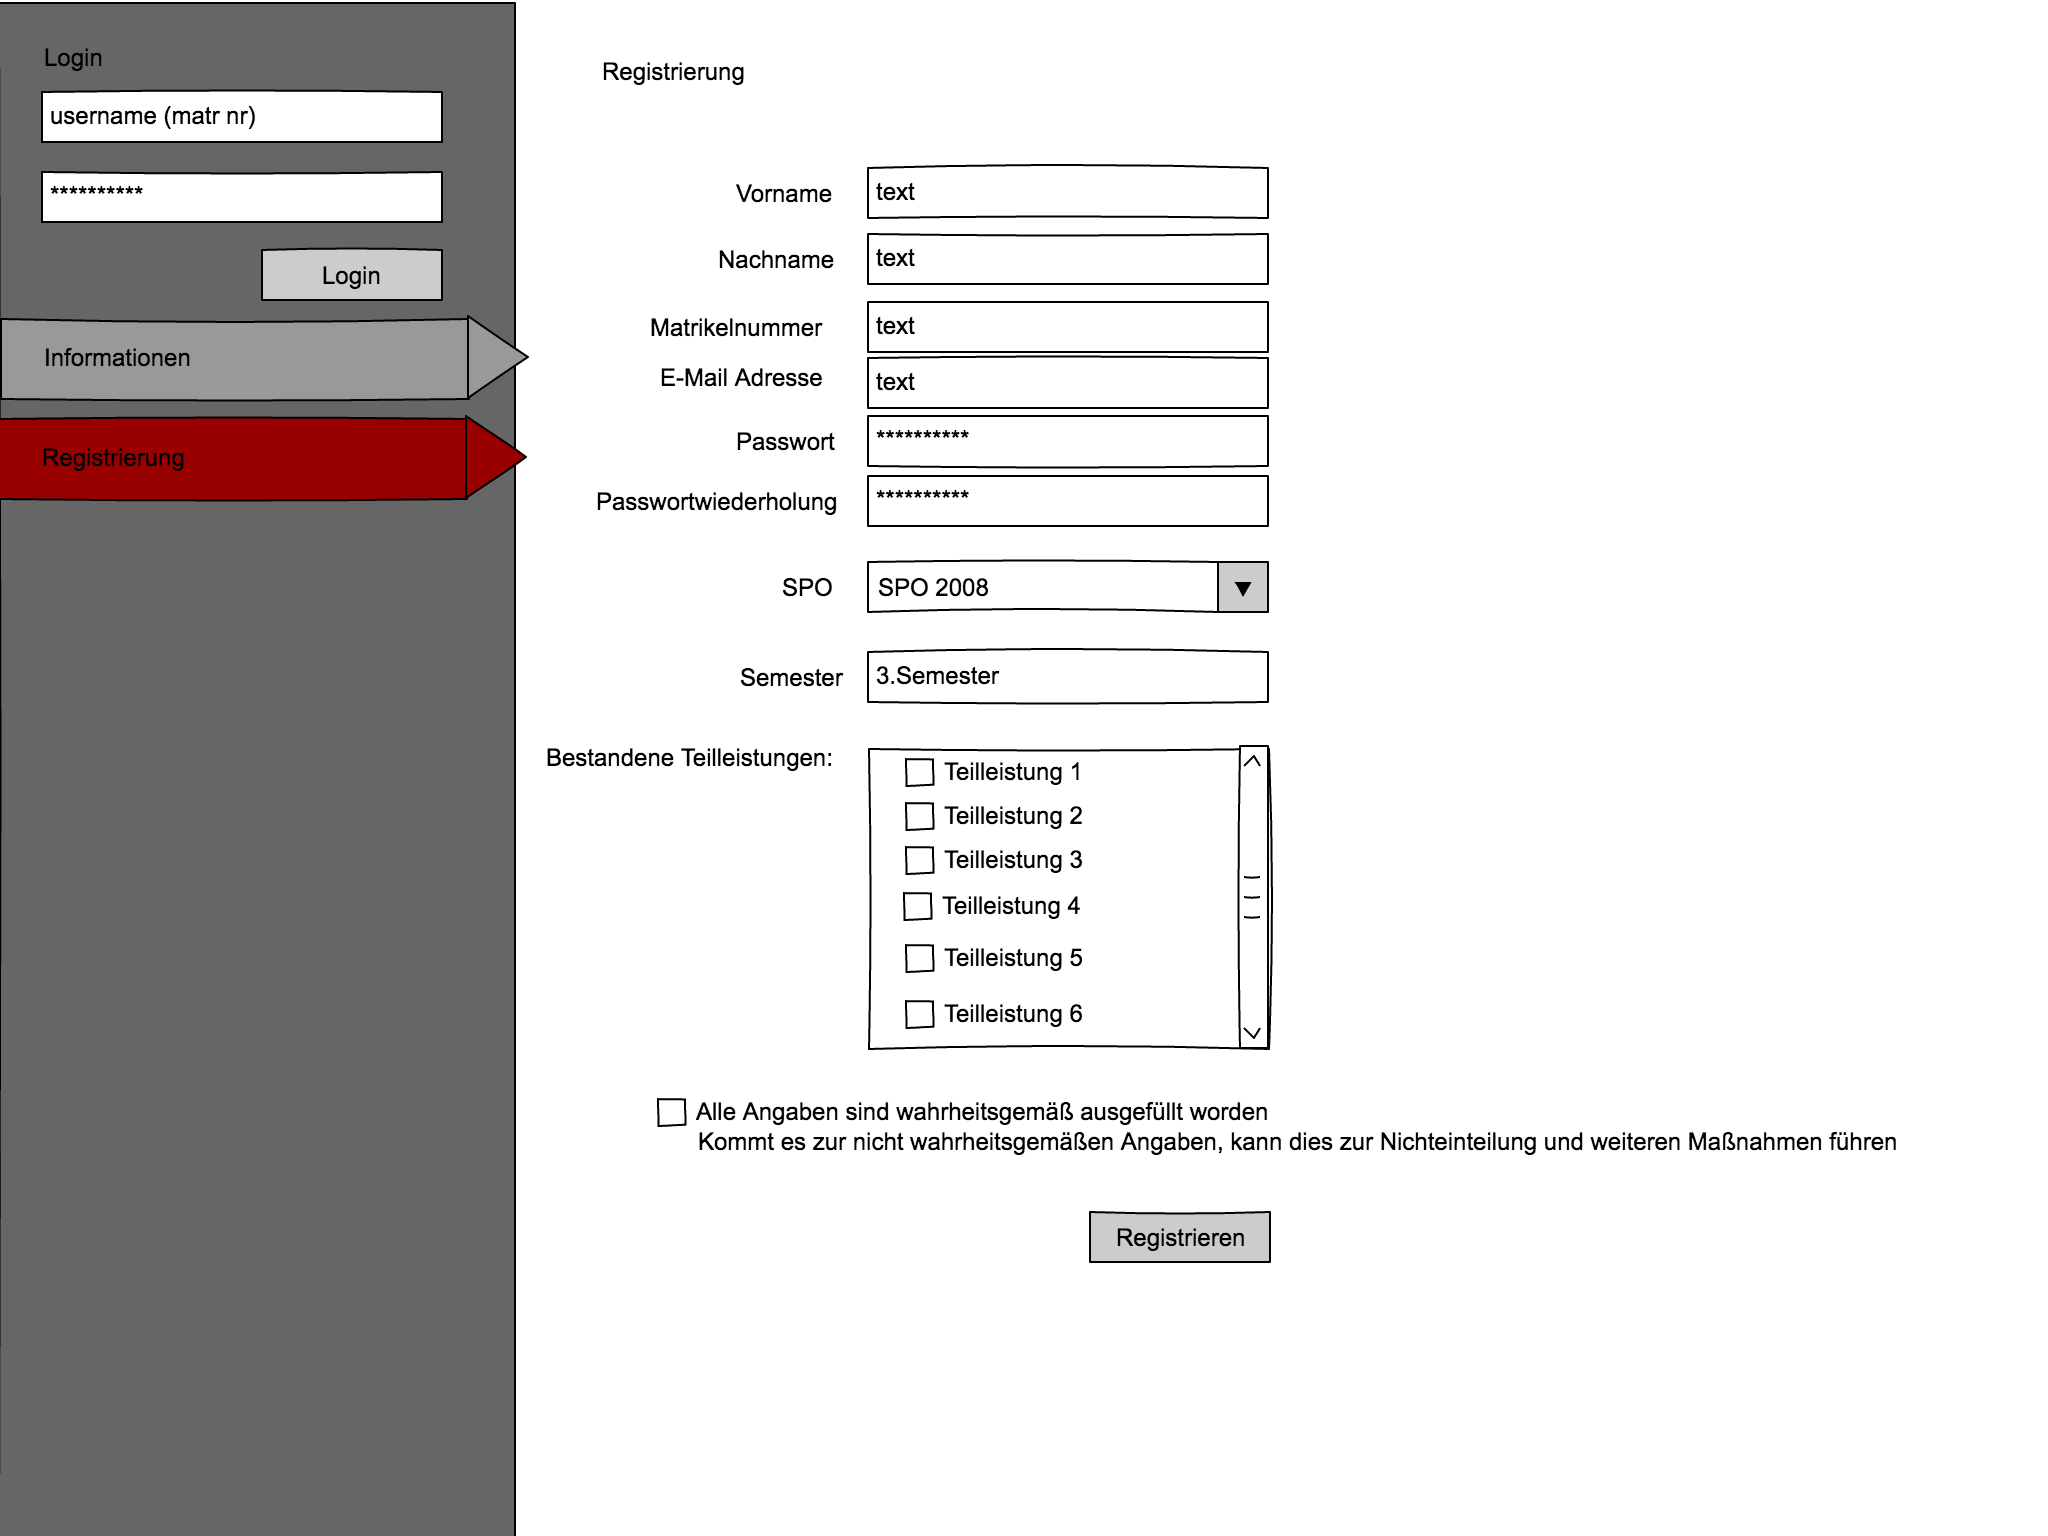
\includegraphics[width=\textwidth,
keepaspectratio=true]{gui/registrierung.png}}
\captionof{figure}{Registrierungsansicht} \label{GUIregi}
\thispagestyle{empty}

\fbox{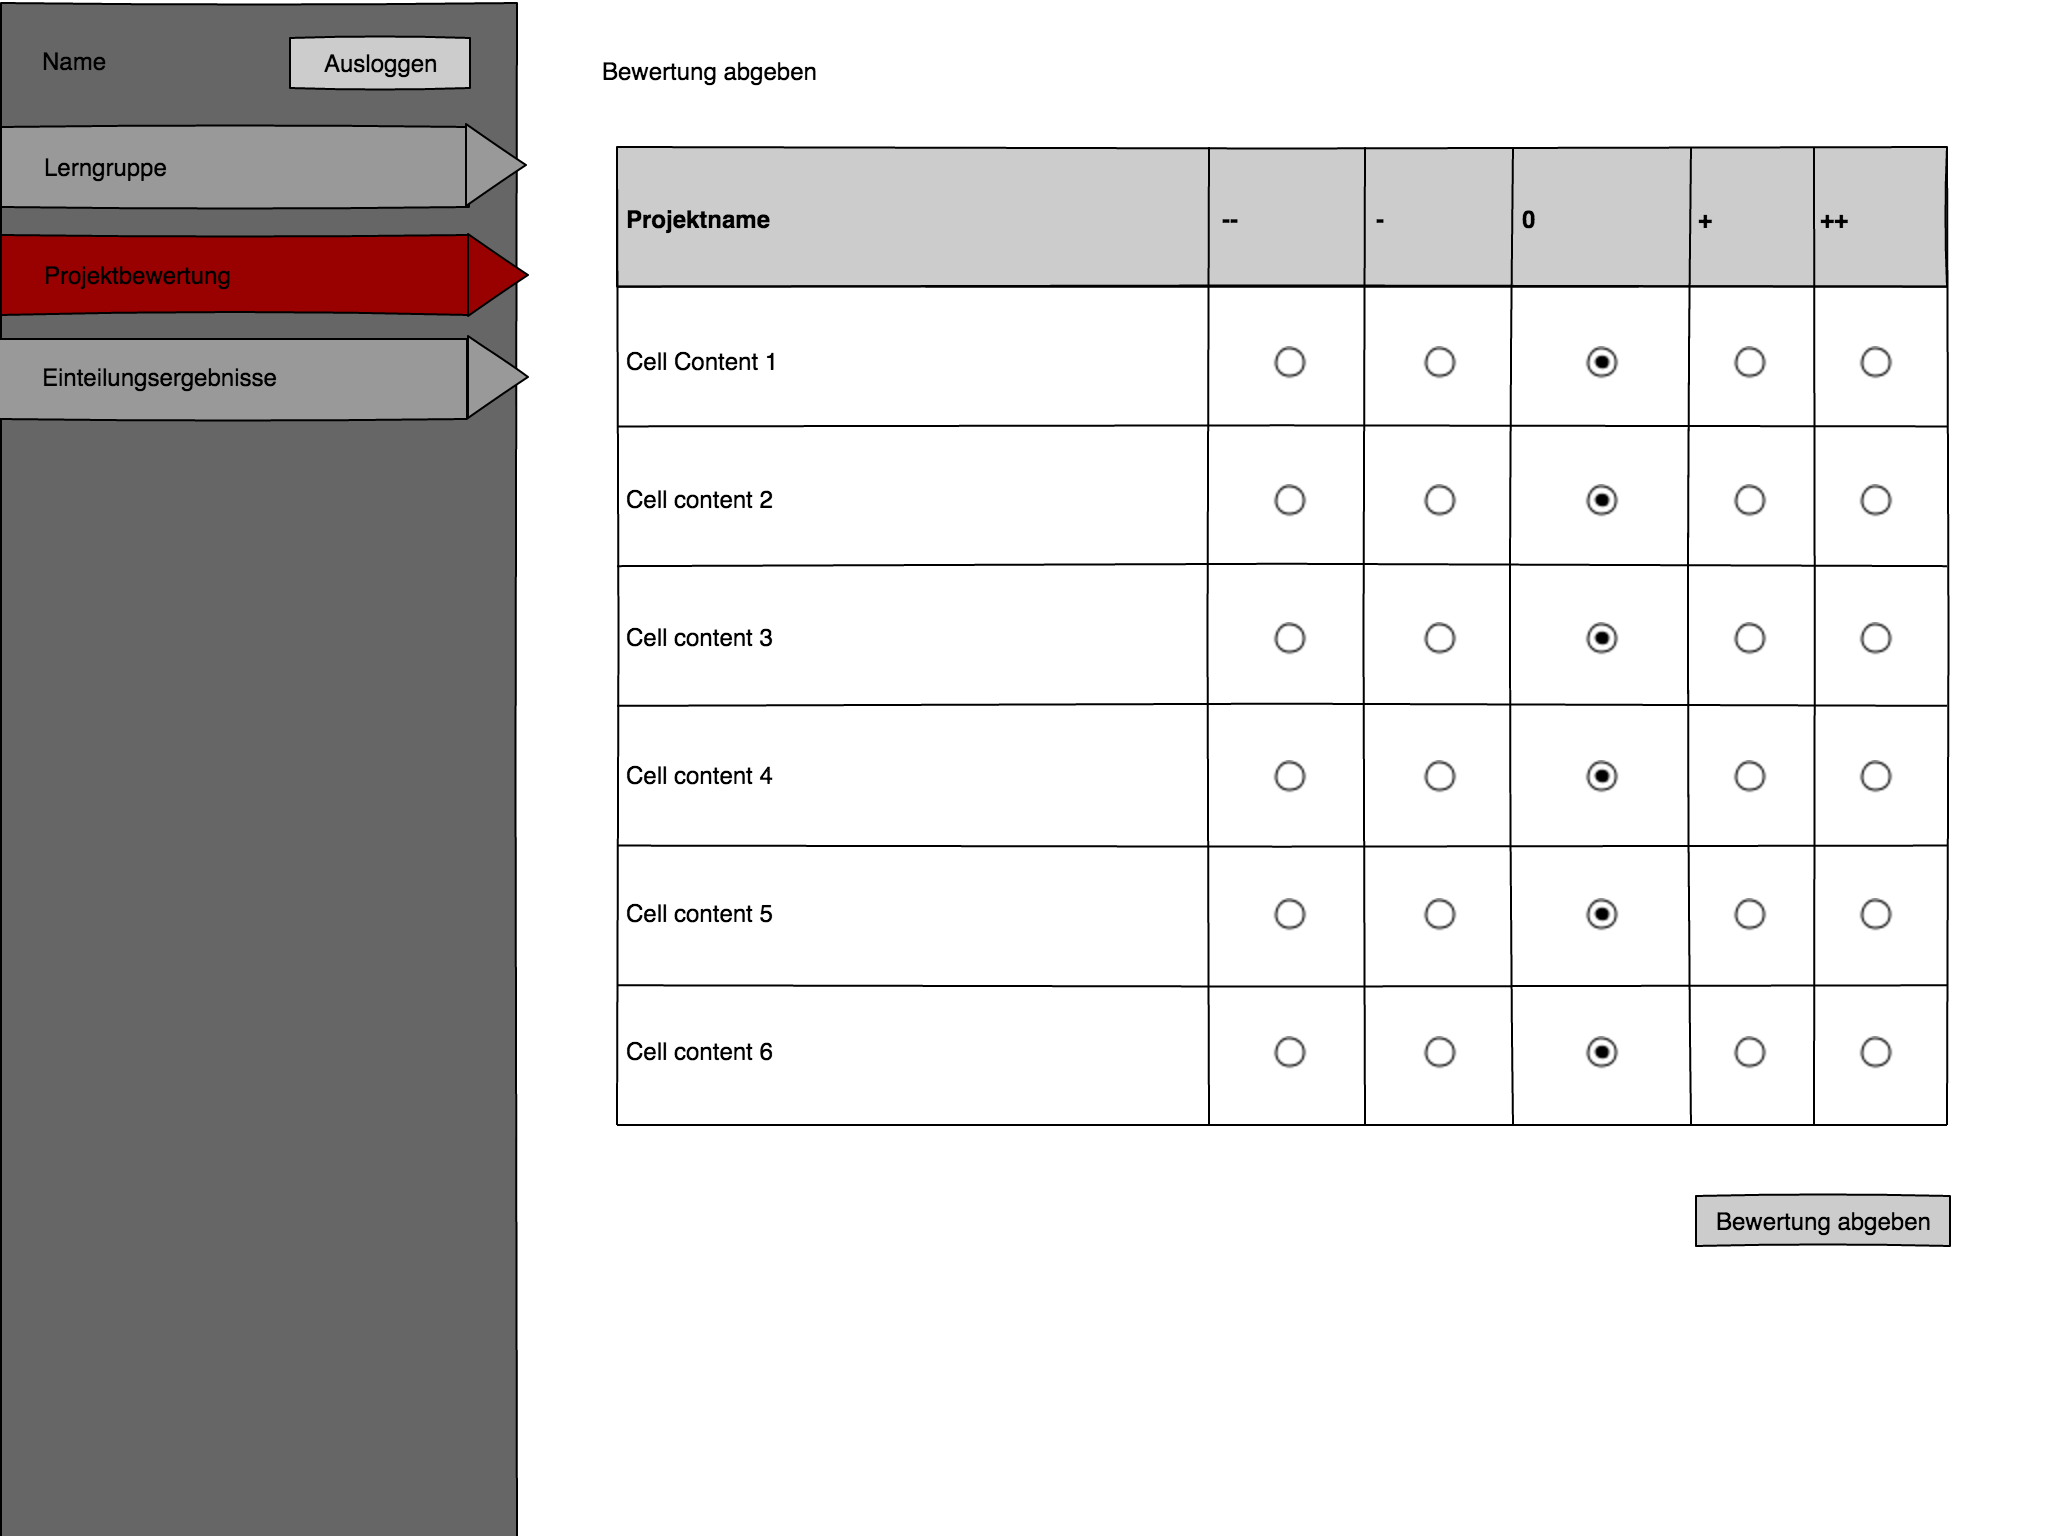
\includegraphics[width=\textwidth,
keepaspectratio=true]{gui/studentbewertung.png}}
\captionof{figure}{Bewertungsmaske} \label{GUIbewertung}

\fbox{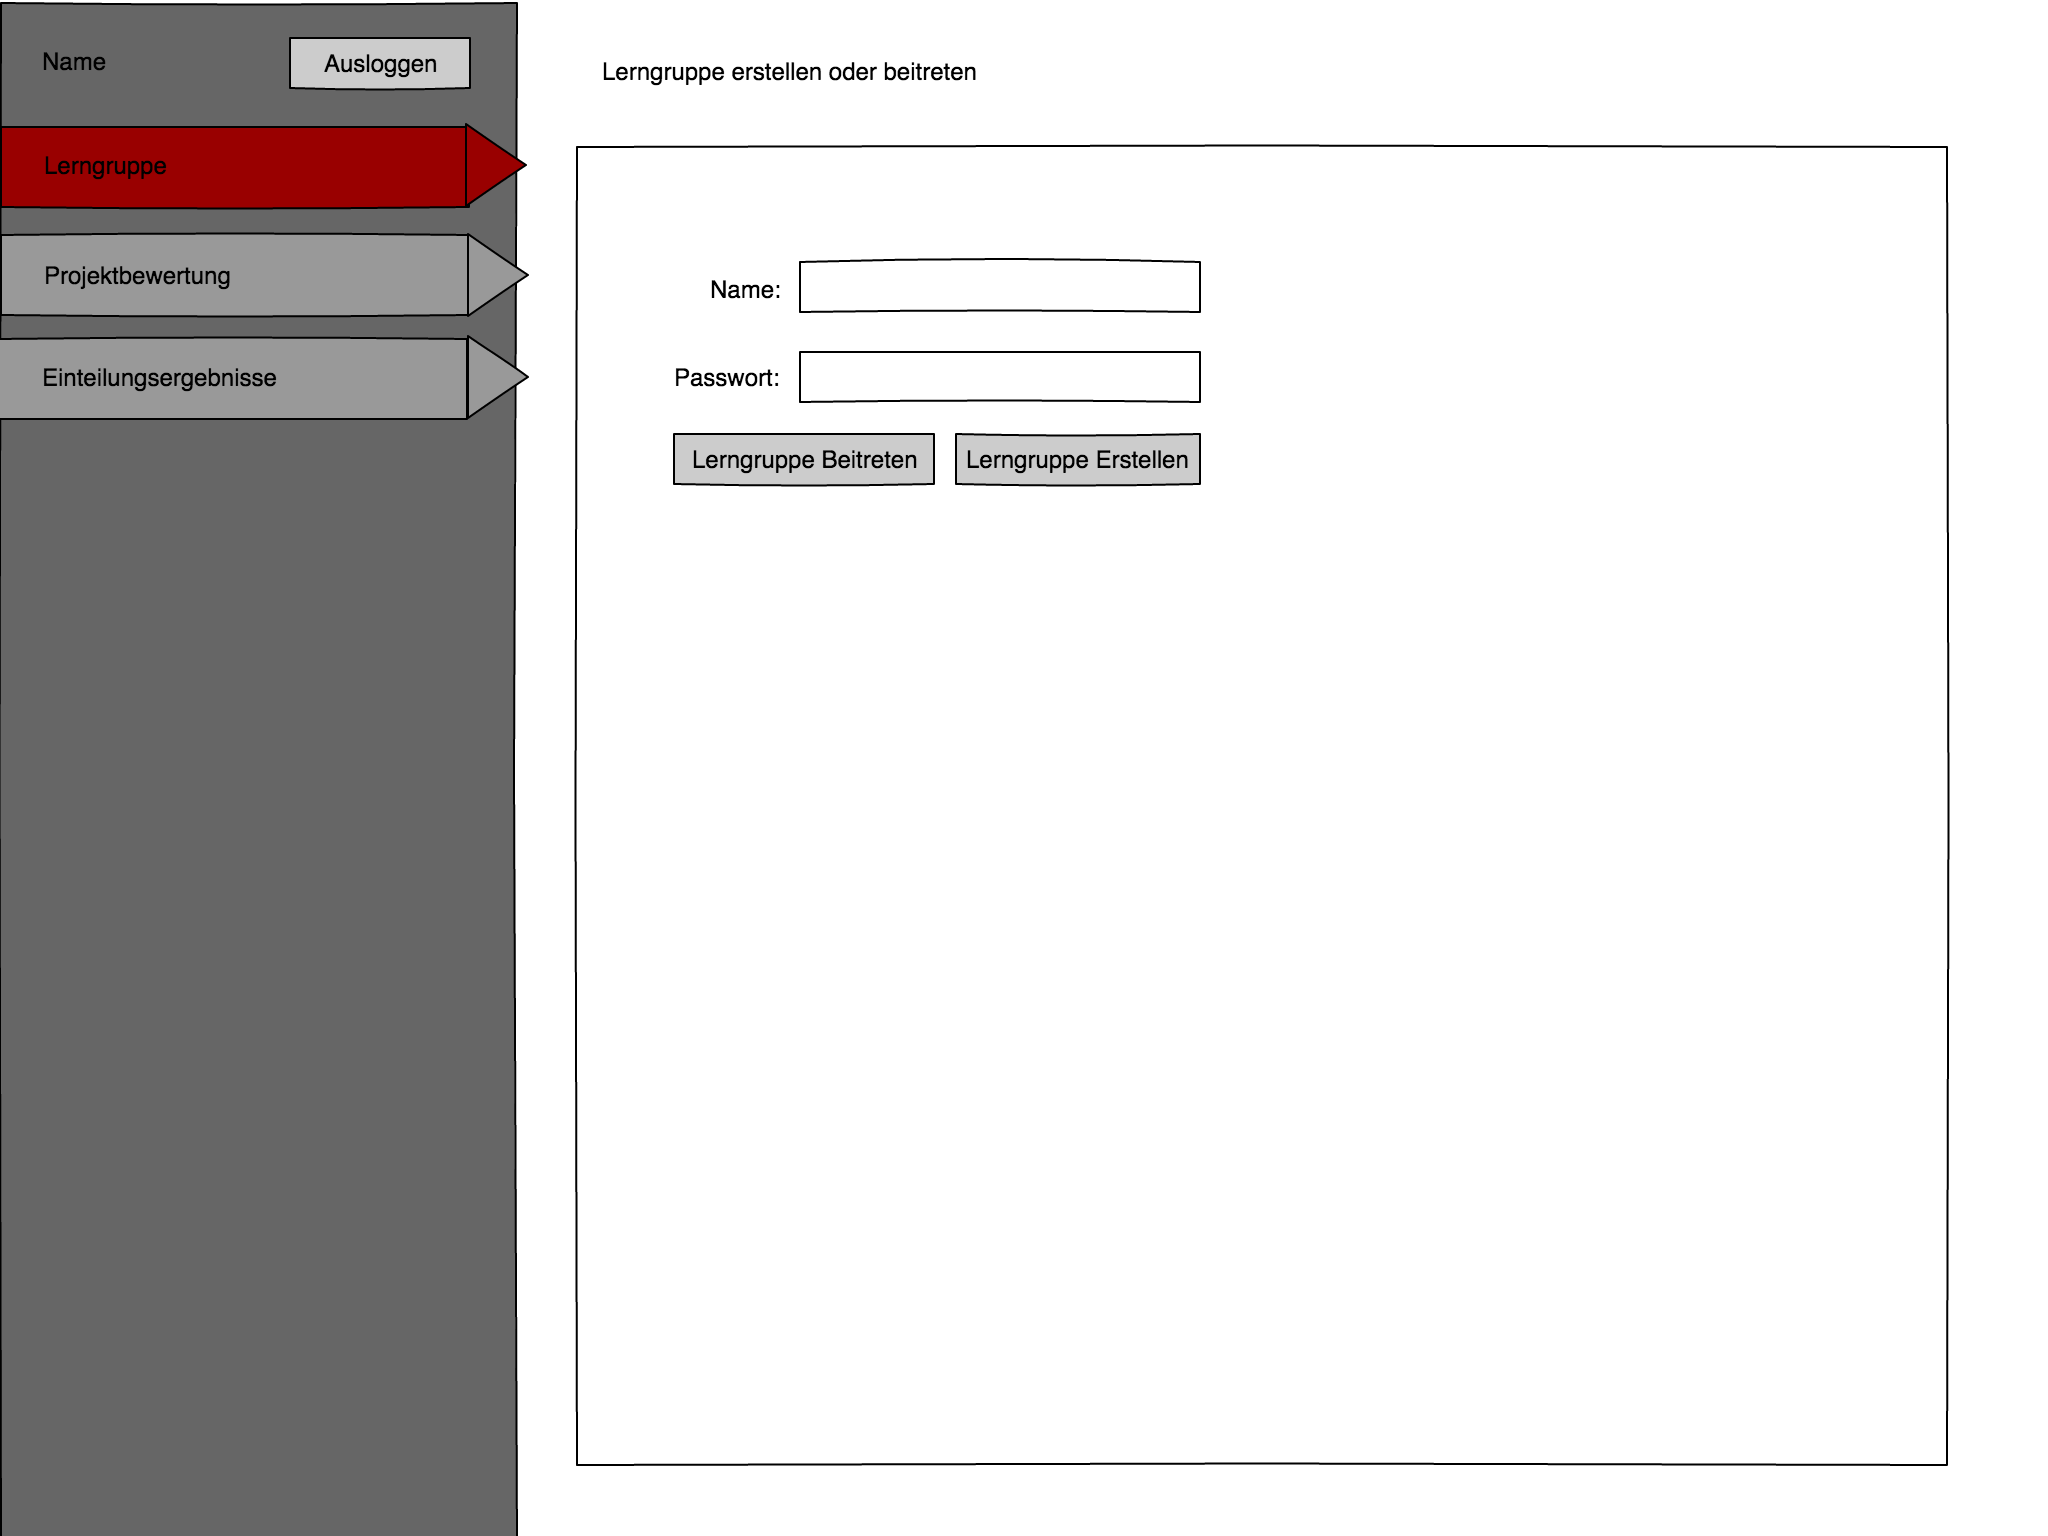
\includegraphics[width=\textwidth,
keepaspectratio=true]{gui/studentlerngruppe.png}}
\captionof{figure}{Anmeldung zu Lerngruppe} \label{GUIanmeldLG}
\medskip
\fbox{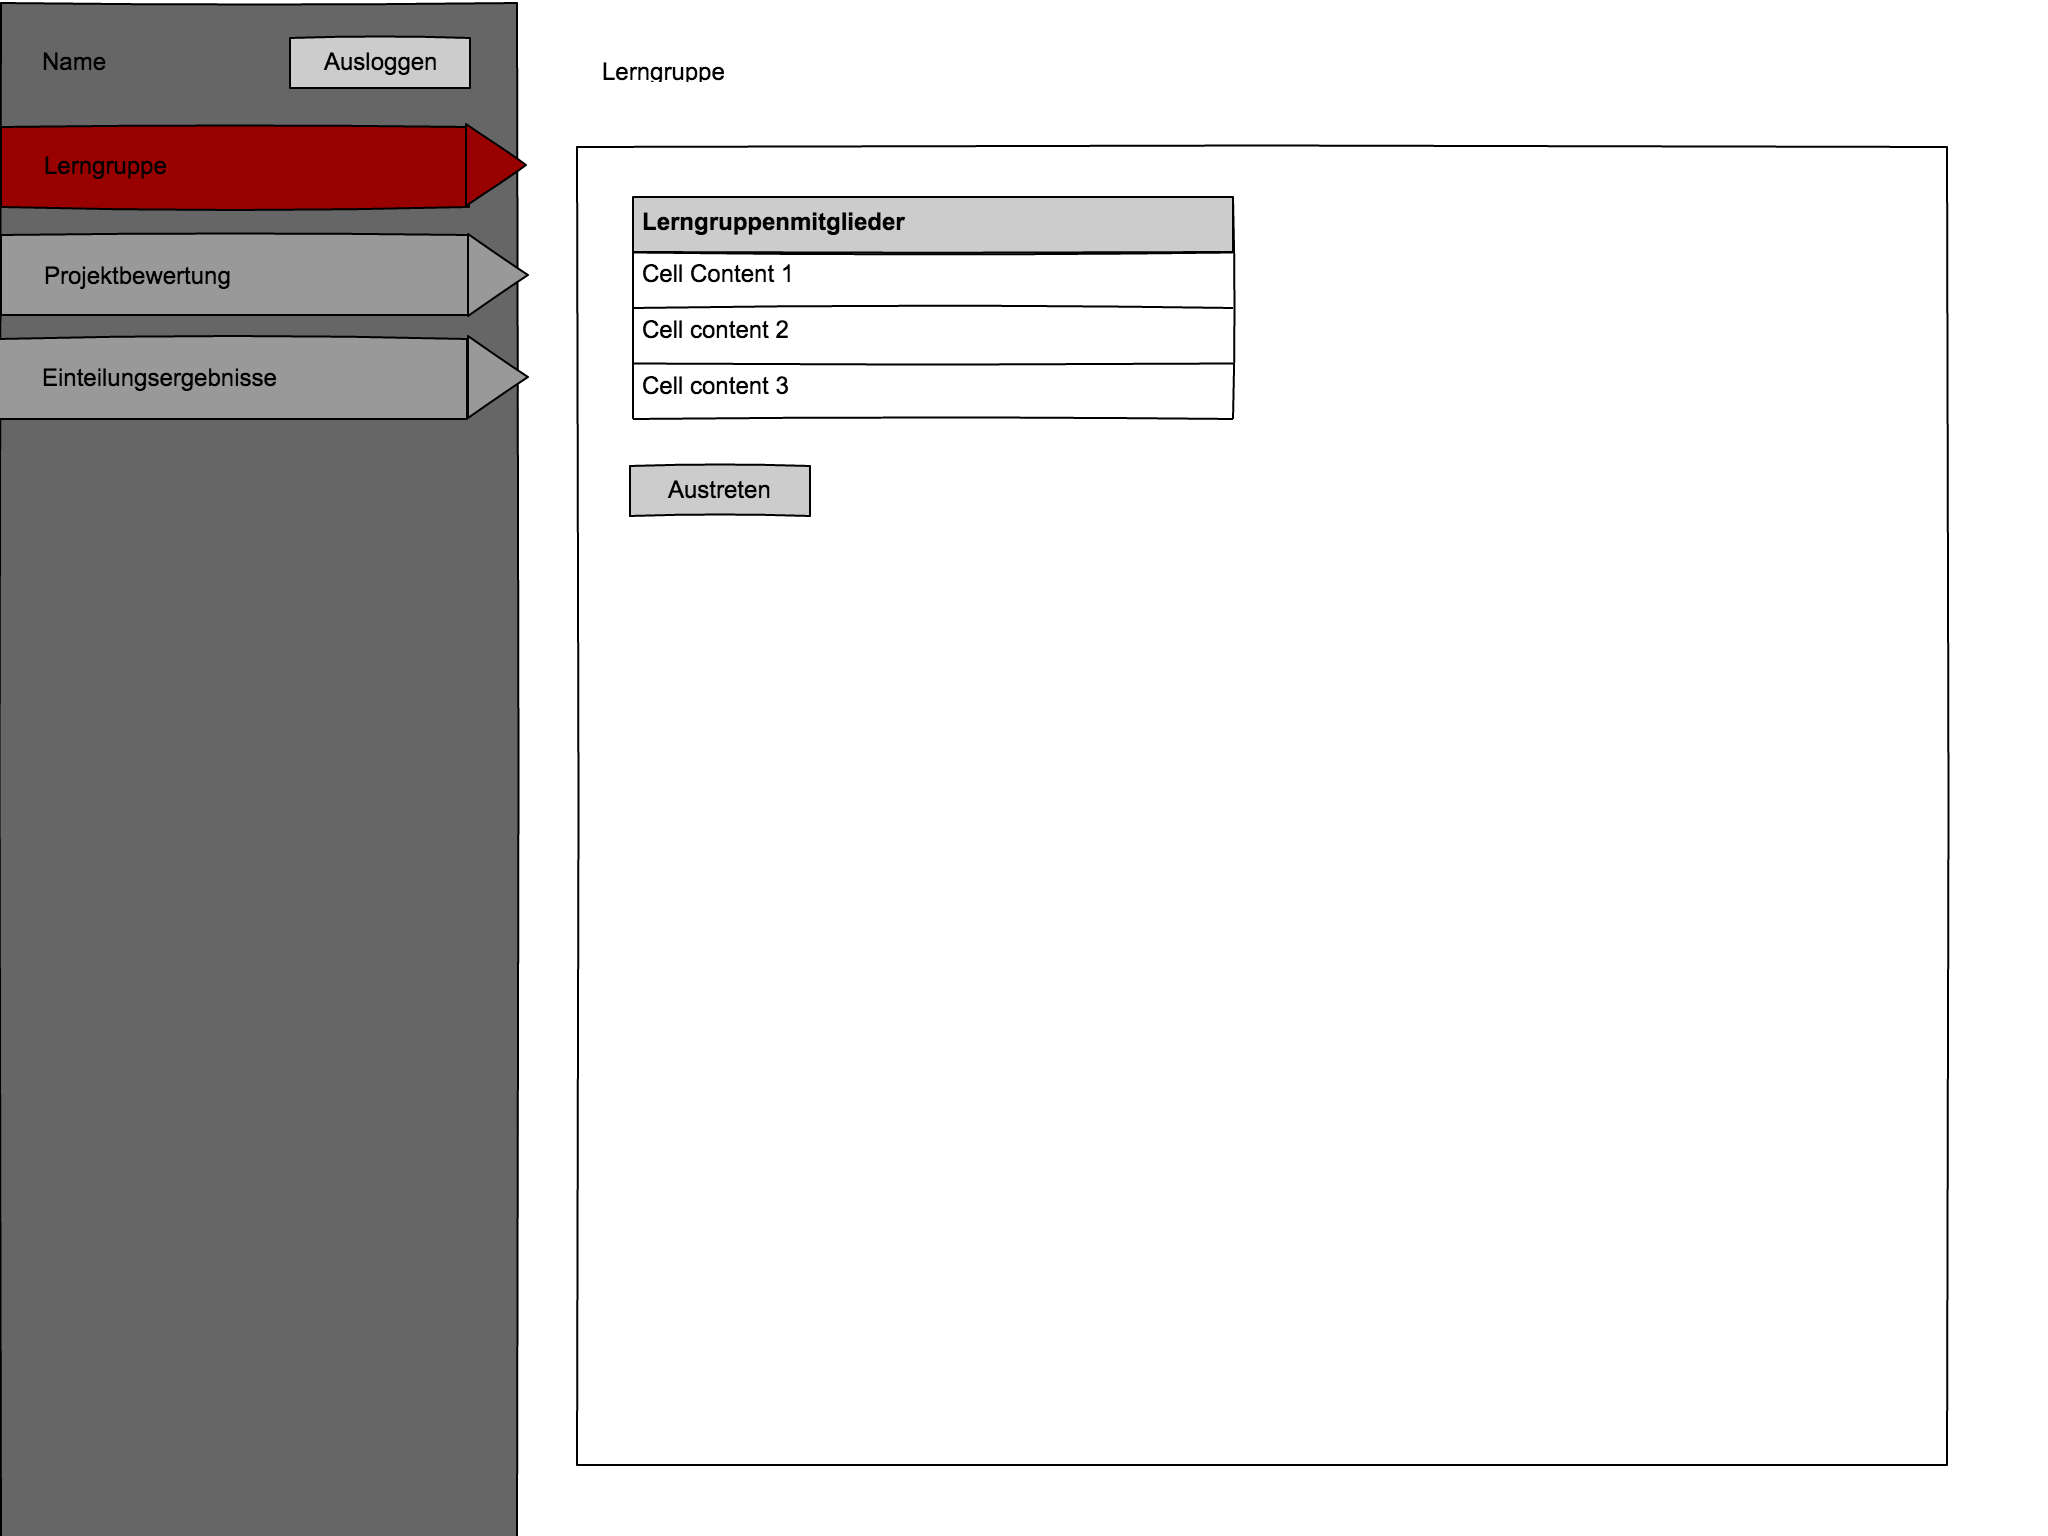
\includegraphics[width=\textwidth,
keepaspectratio=true]{gui/studentlerngruppeingr.png}}
\captionof{figure}{Lerngruppenübersicht} \label{GUIlerngUebersicht}
\medskip
\fbox{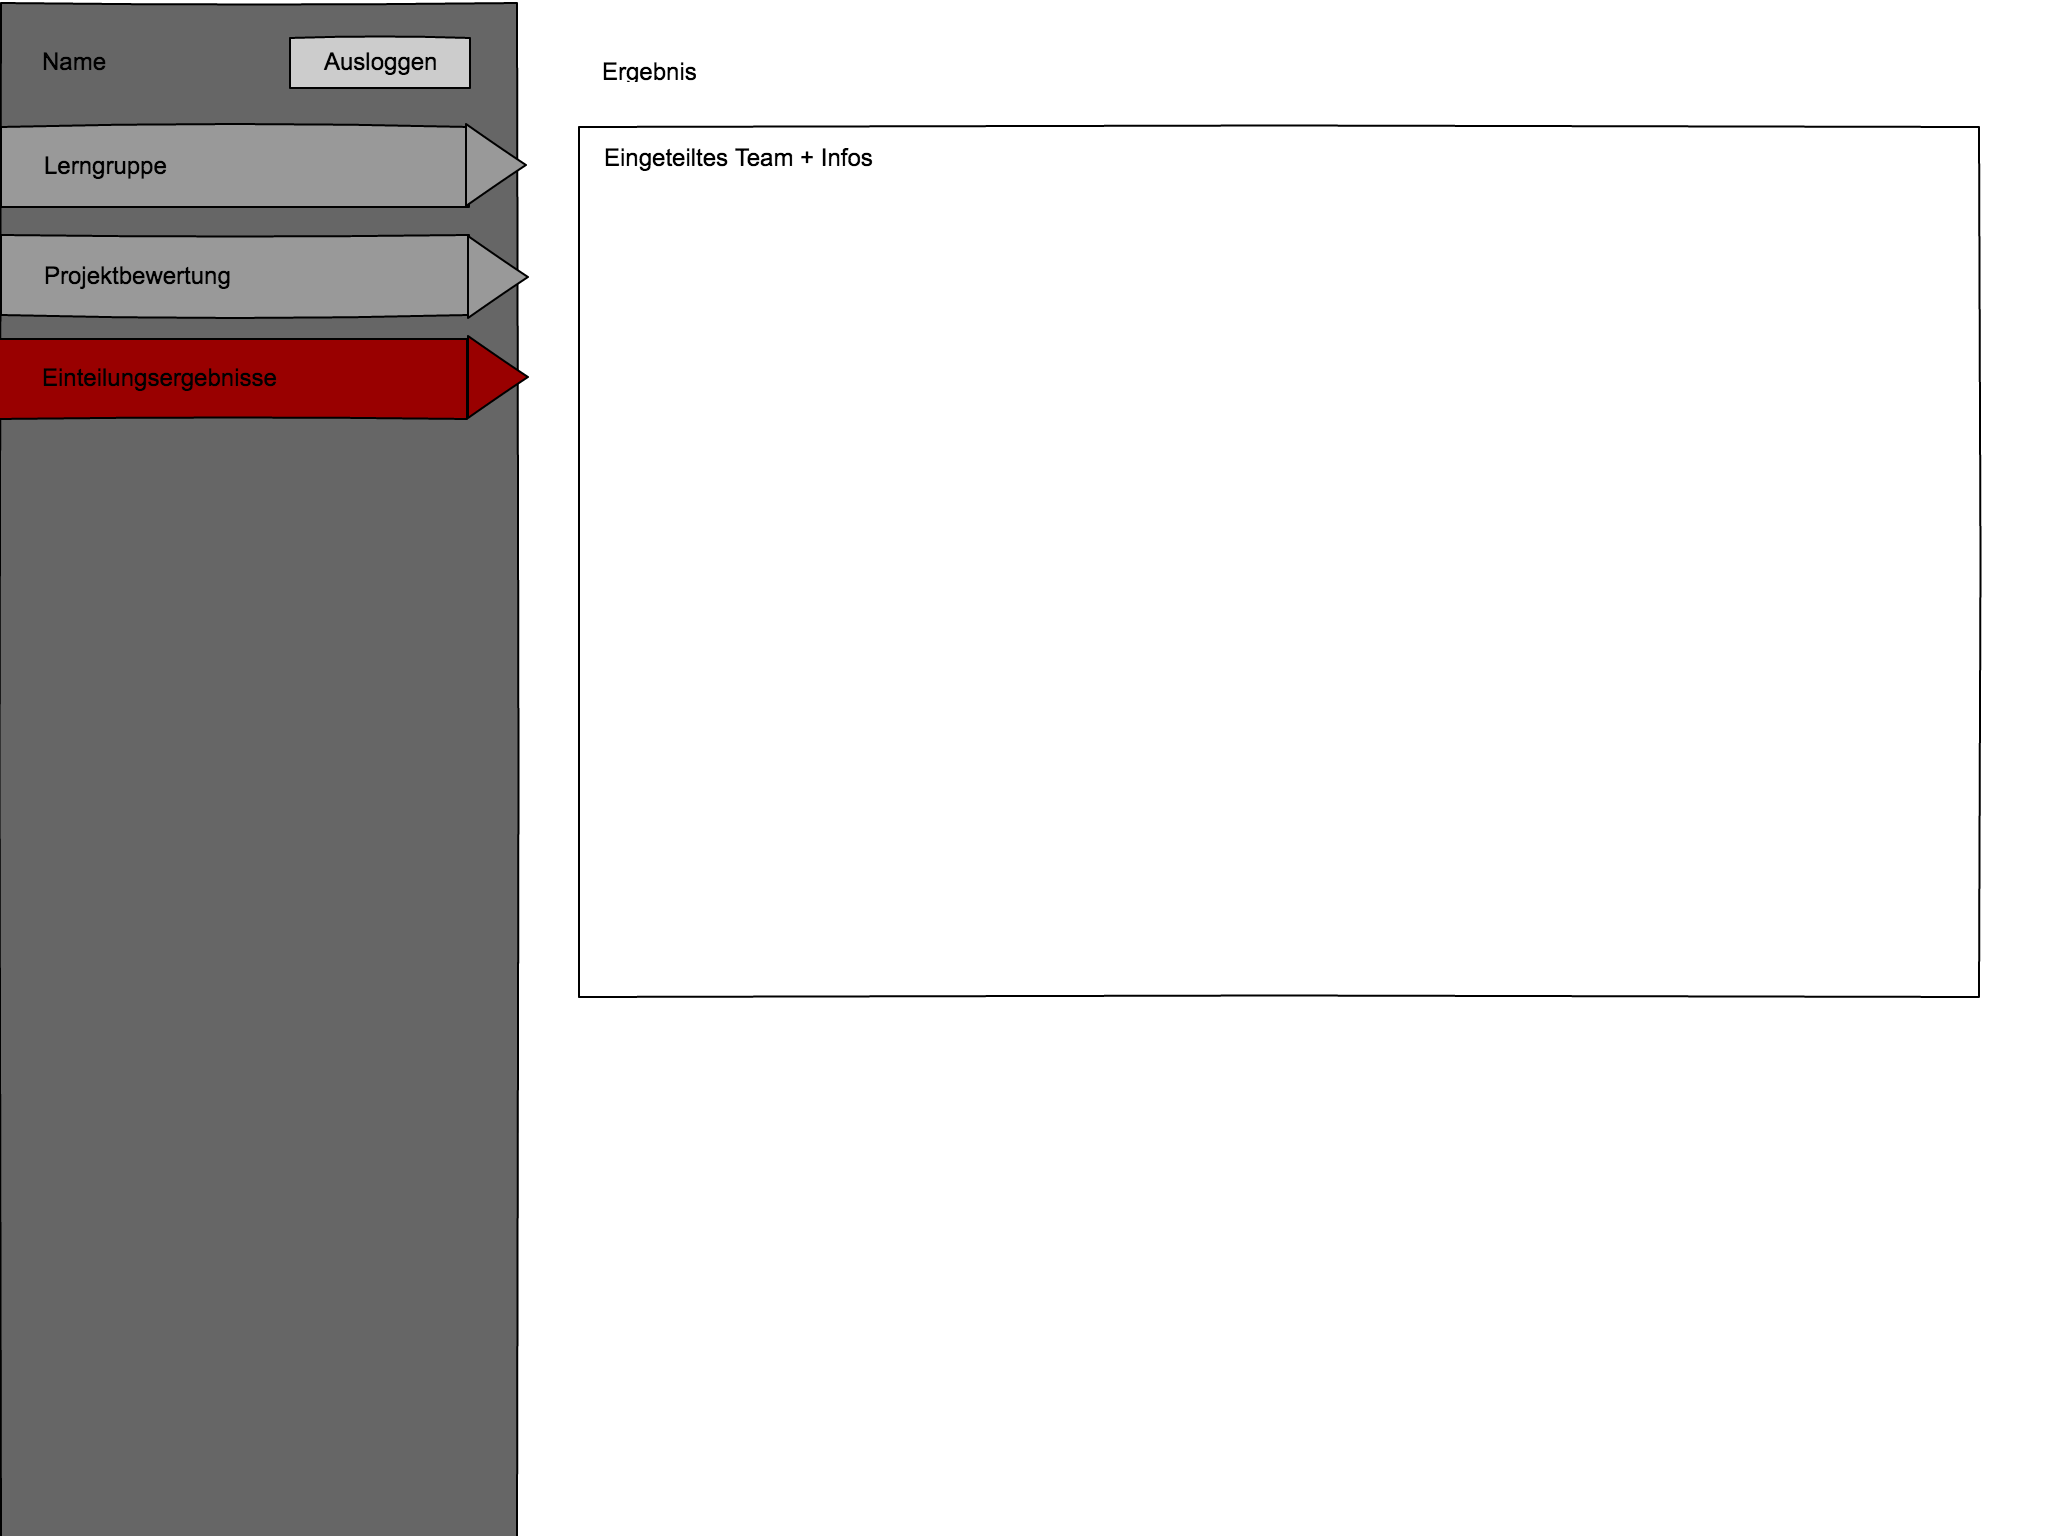
\includegraphics[width=\textwidth,
keepaspectratio=true]{gui/studentergebnis.png}}
\captionof{figure}{Ergebnisansicht} \label{GUIergebnisAnsicht}
\medskip
\fbox{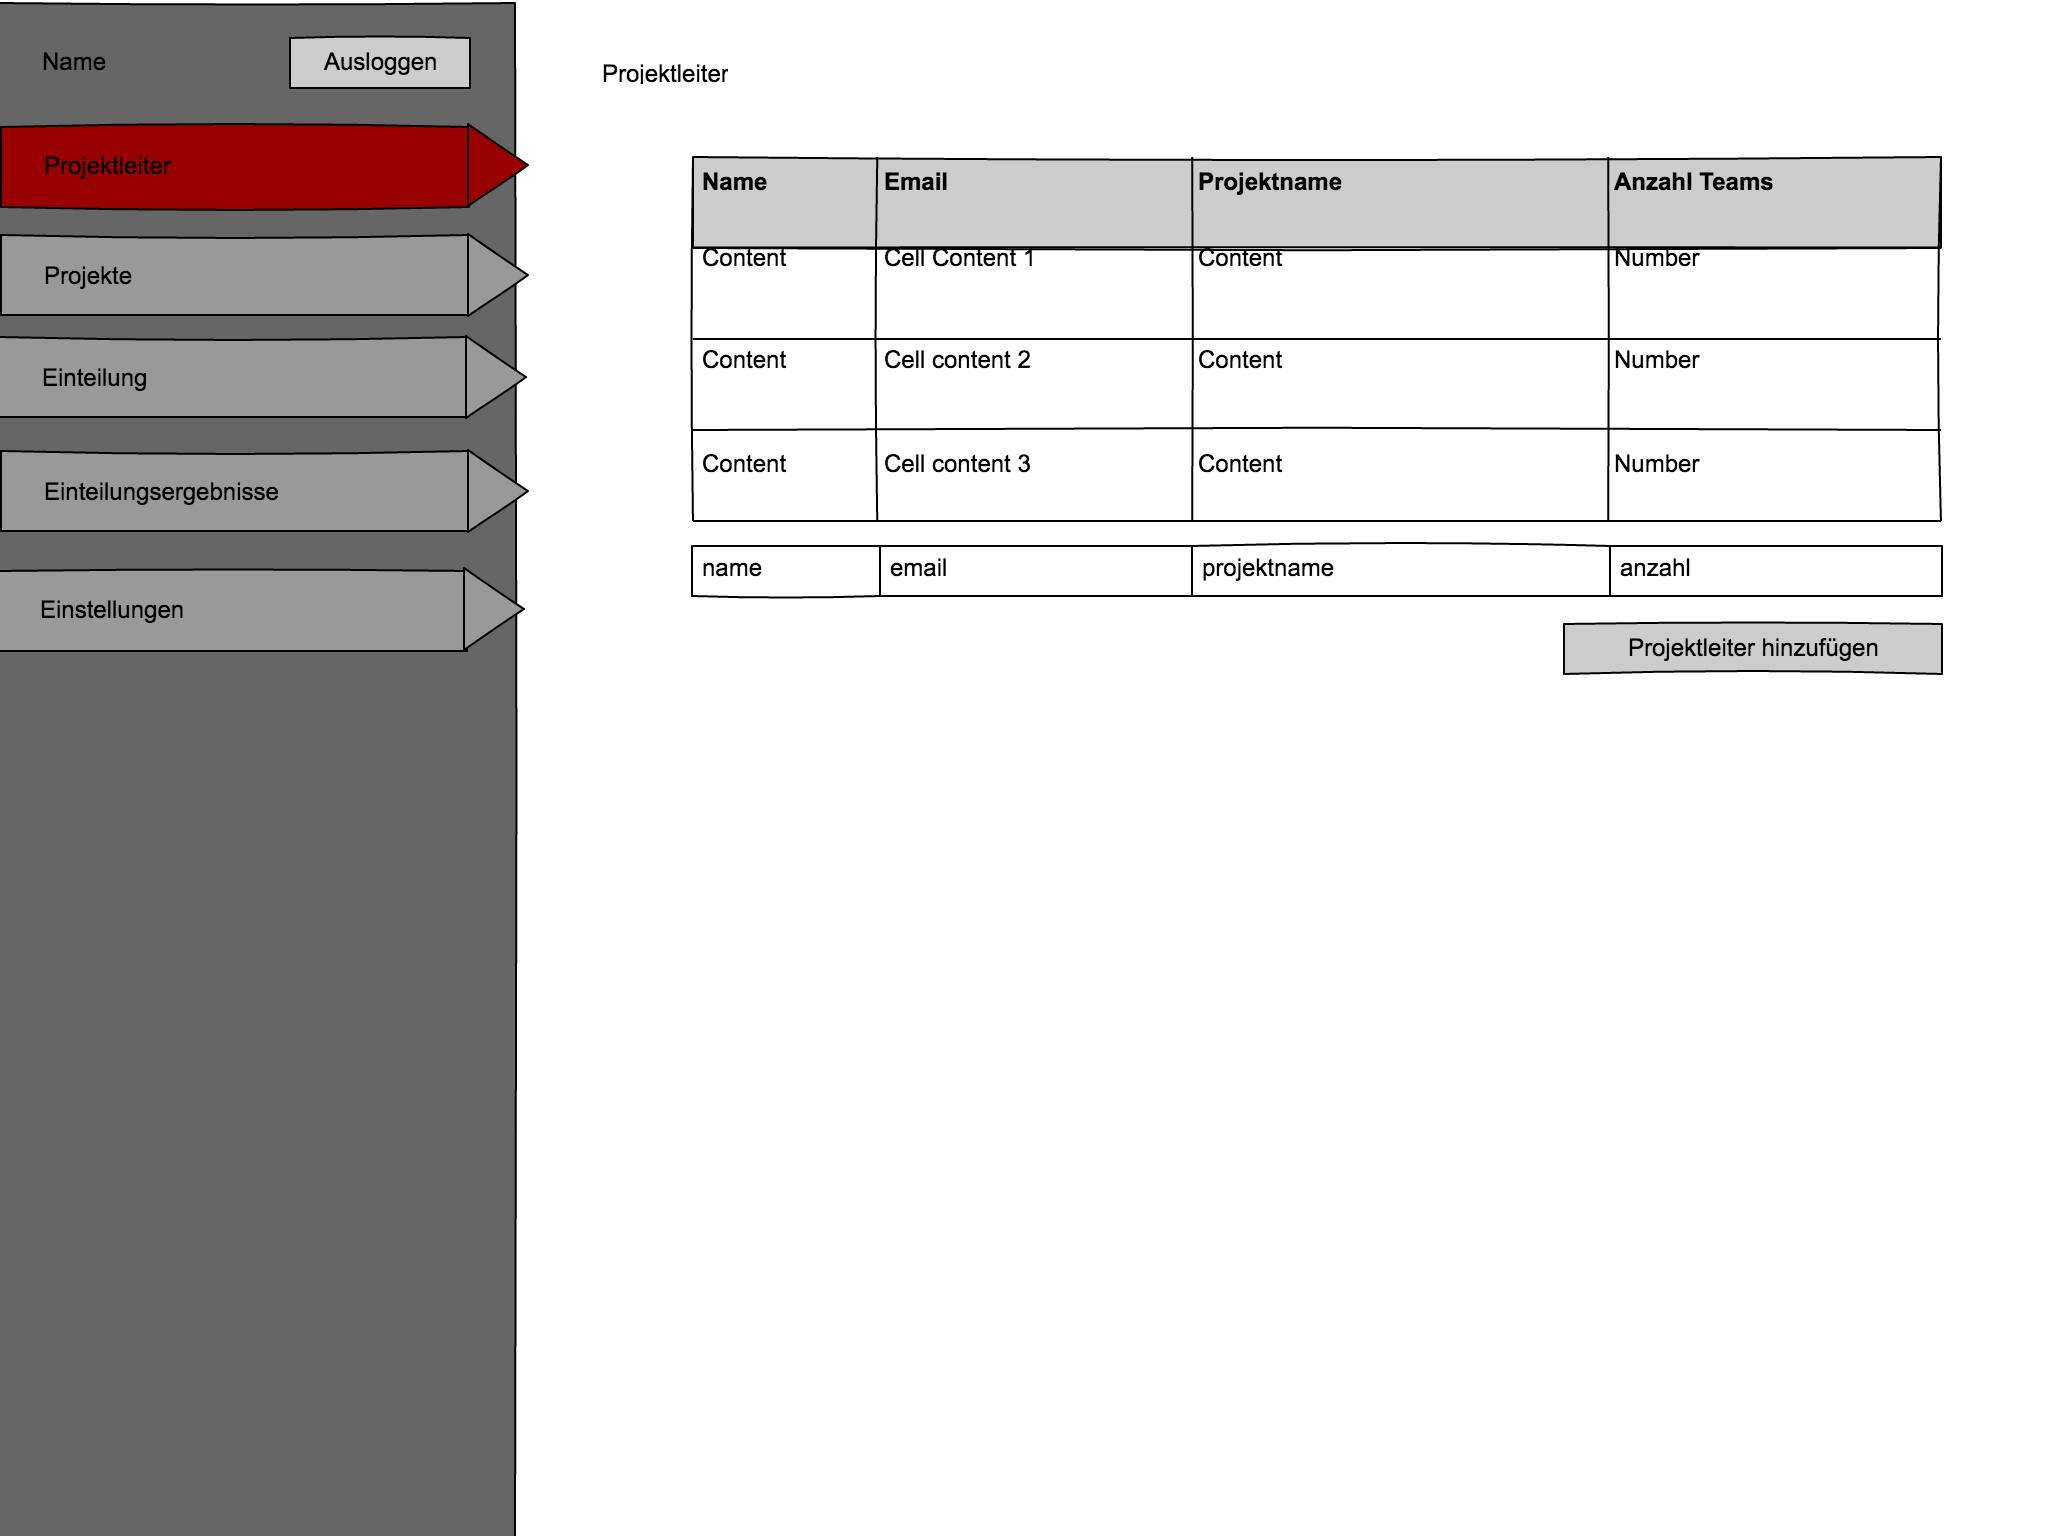
\includegraphics[width=\textwidth,
keepaspectratio=true]{gui/adminprojleiter.png}}
\captionof{figure}{Projektleiterübersicht} \label{GUIprojLeiterUebersicht}
\medskip
\fbox{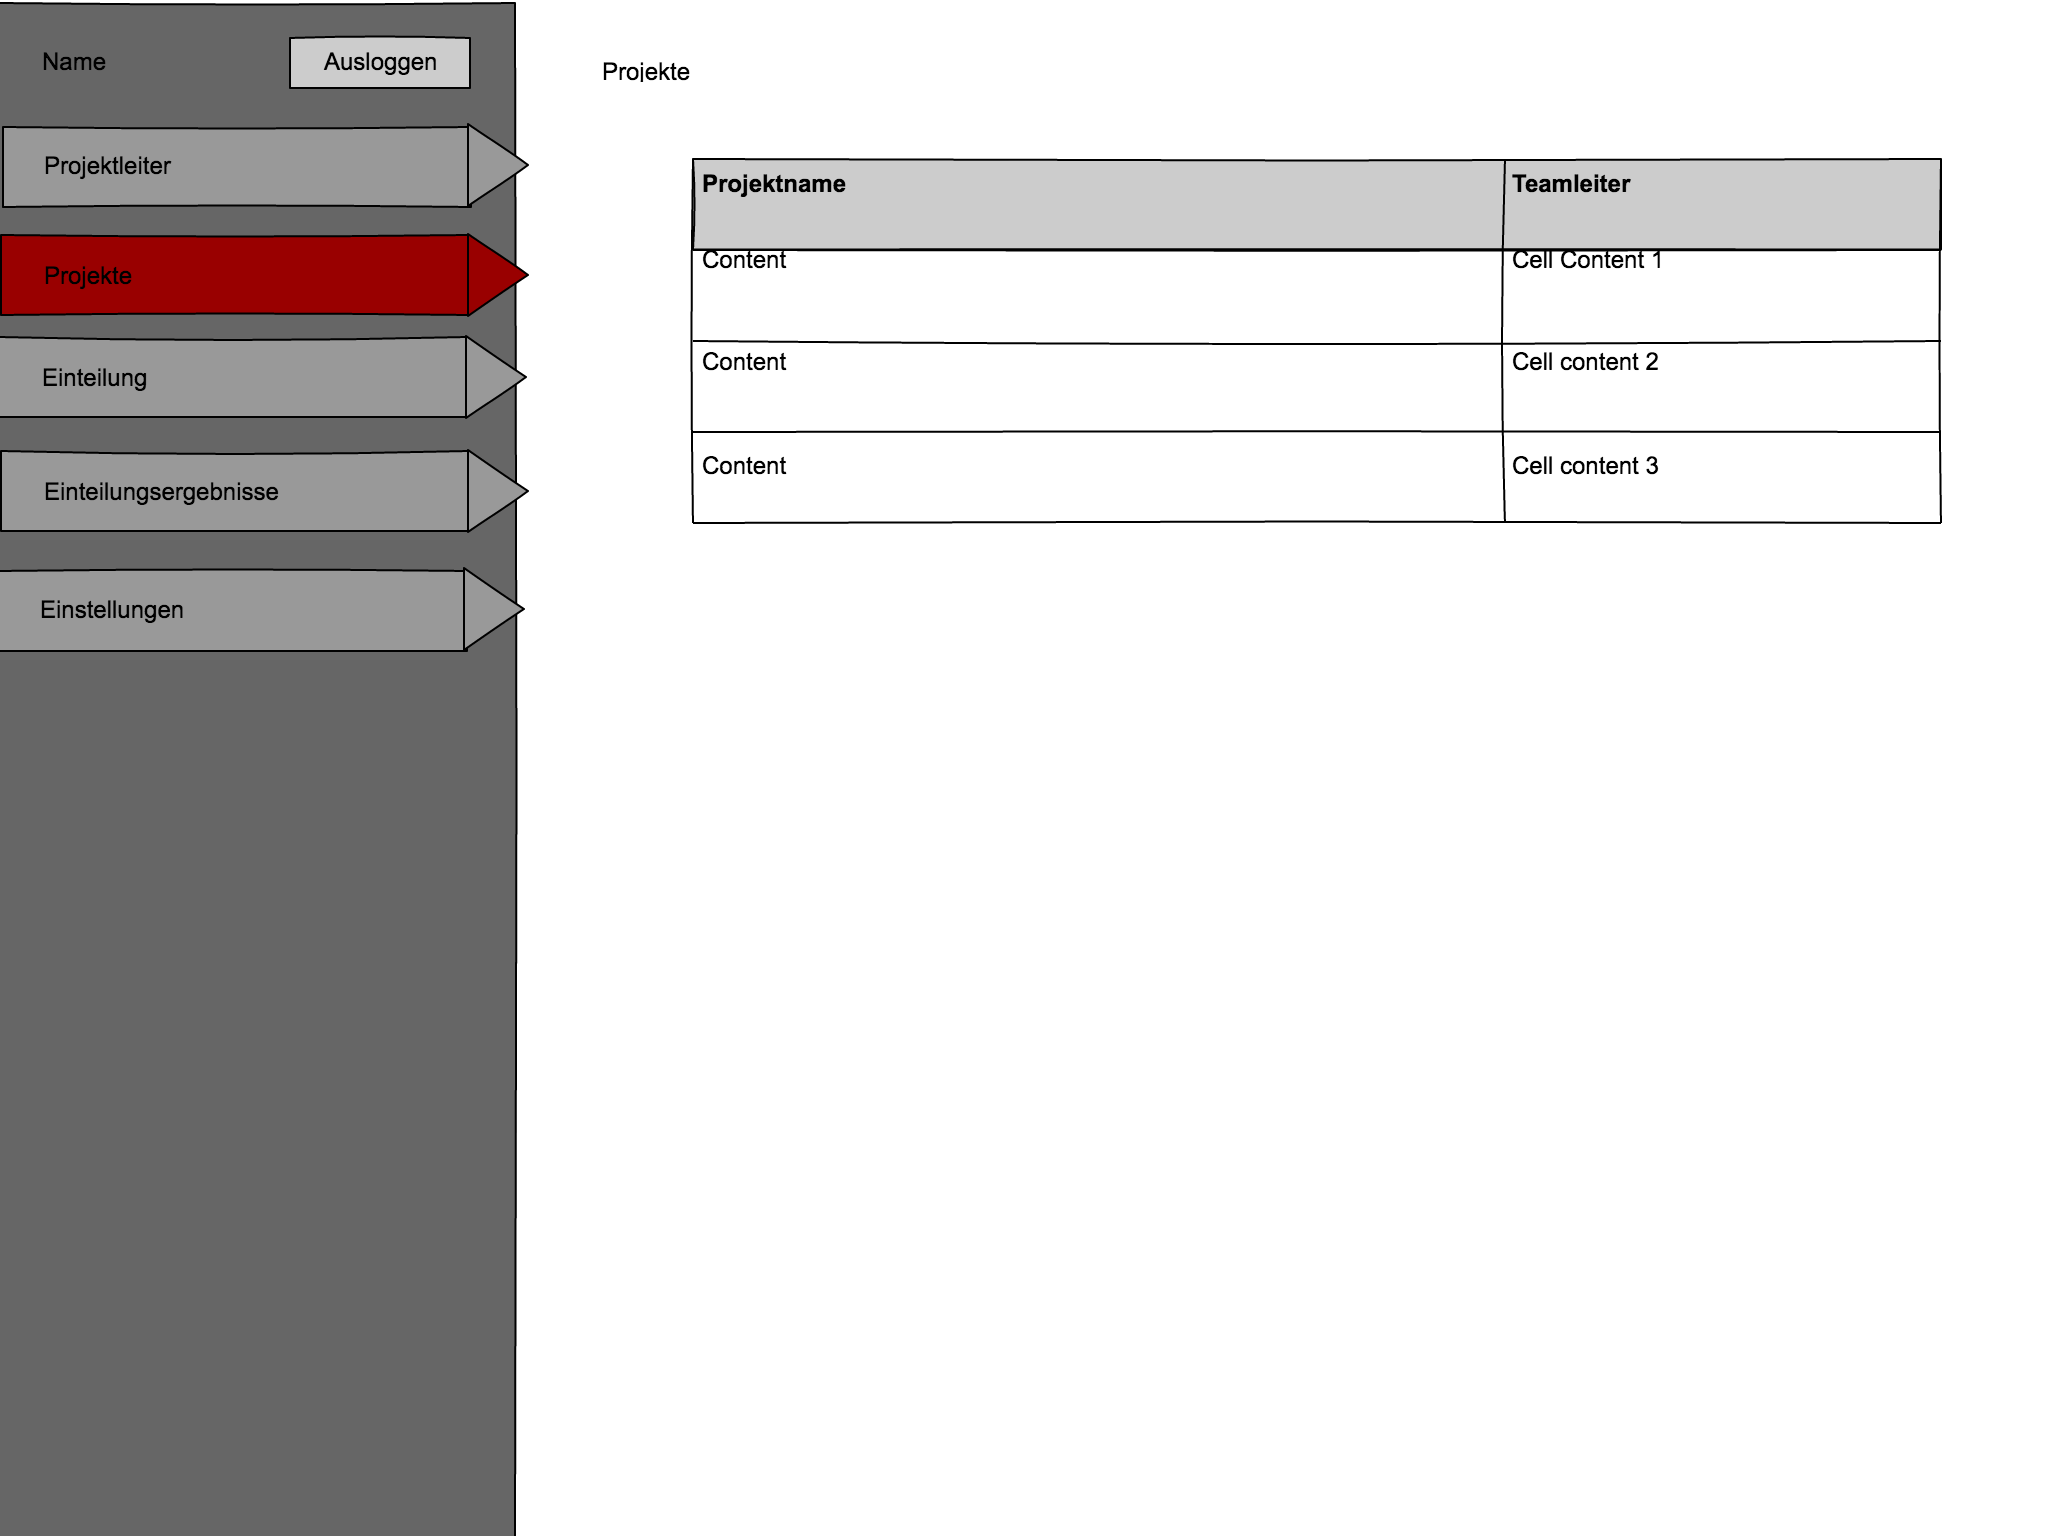
\includegraphics[width=\textwidth,
keepaspectratio=true]{gui/adminprojekte.png}}

\captionof{figure}{Projektübersicht} \label{GUIprojUebersicht}
\medskip
\fbox{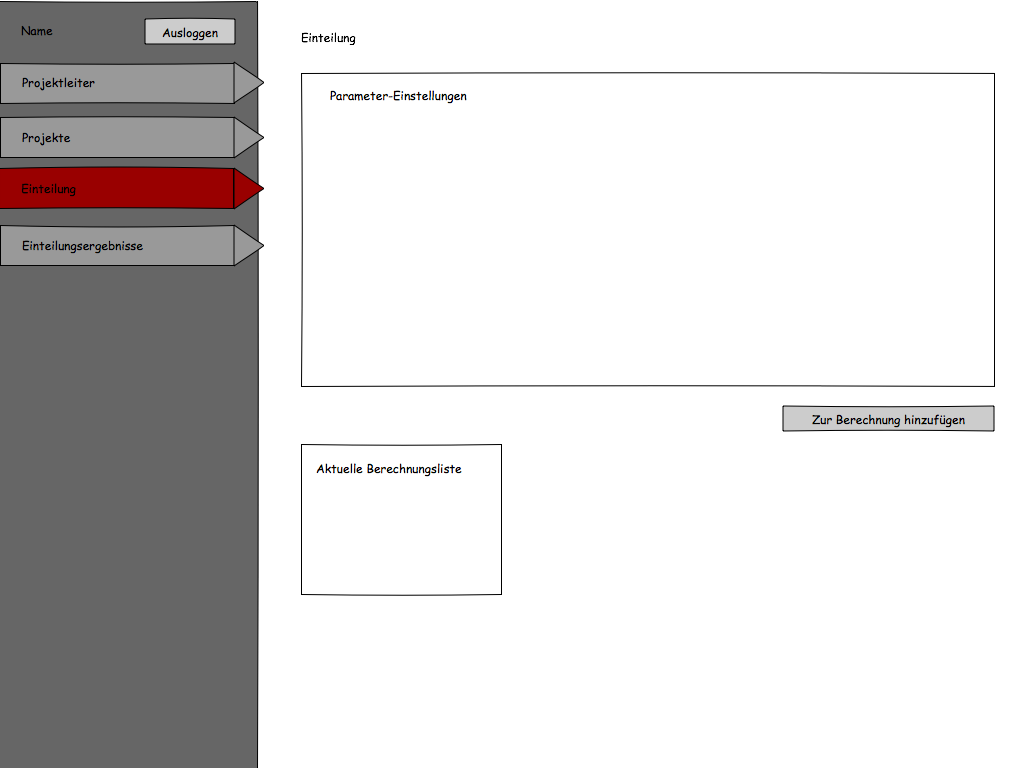
\includegraphics[width=\textwidth,
keepaspectratio=true]{gui/admineinteilung.png}}
\captionof{figure}{Einteilungsmaske} \label{GUIeinteilung}
\medskip
\fbox{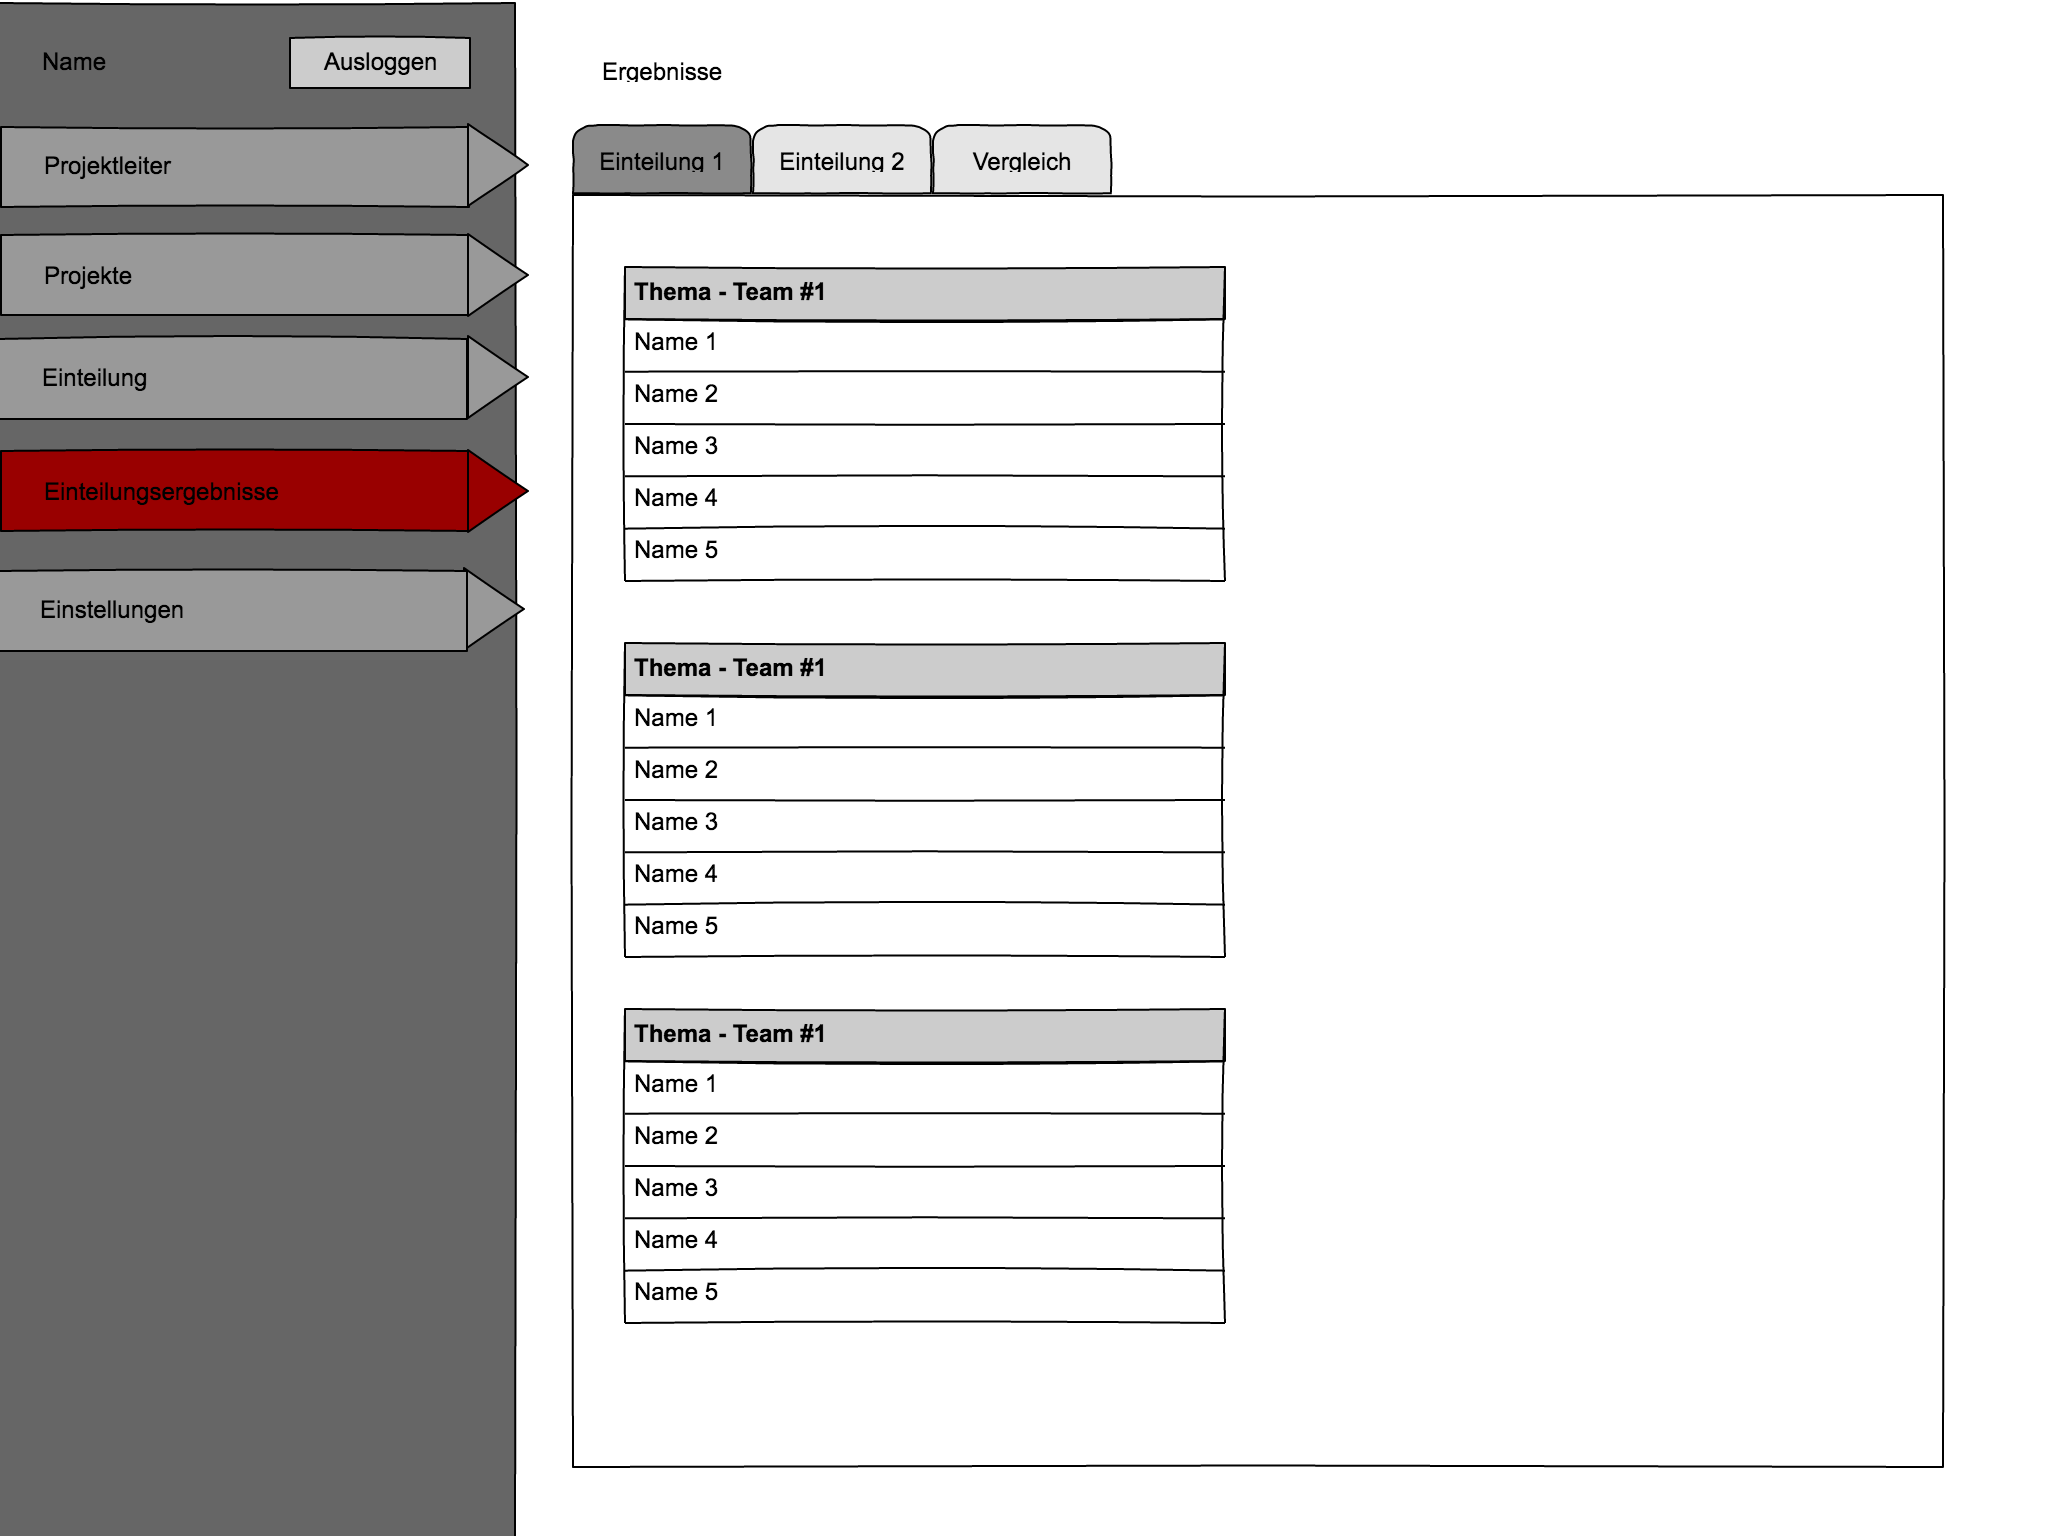
\includegraphics[width=\textwidth,
keepaspectratio=true]{gui/adminergebnisse.png}}
\captionof{figure}{Übersicht der Einteilungen} \label{GUIeinteilungErgeb}
\medskip
\fbox{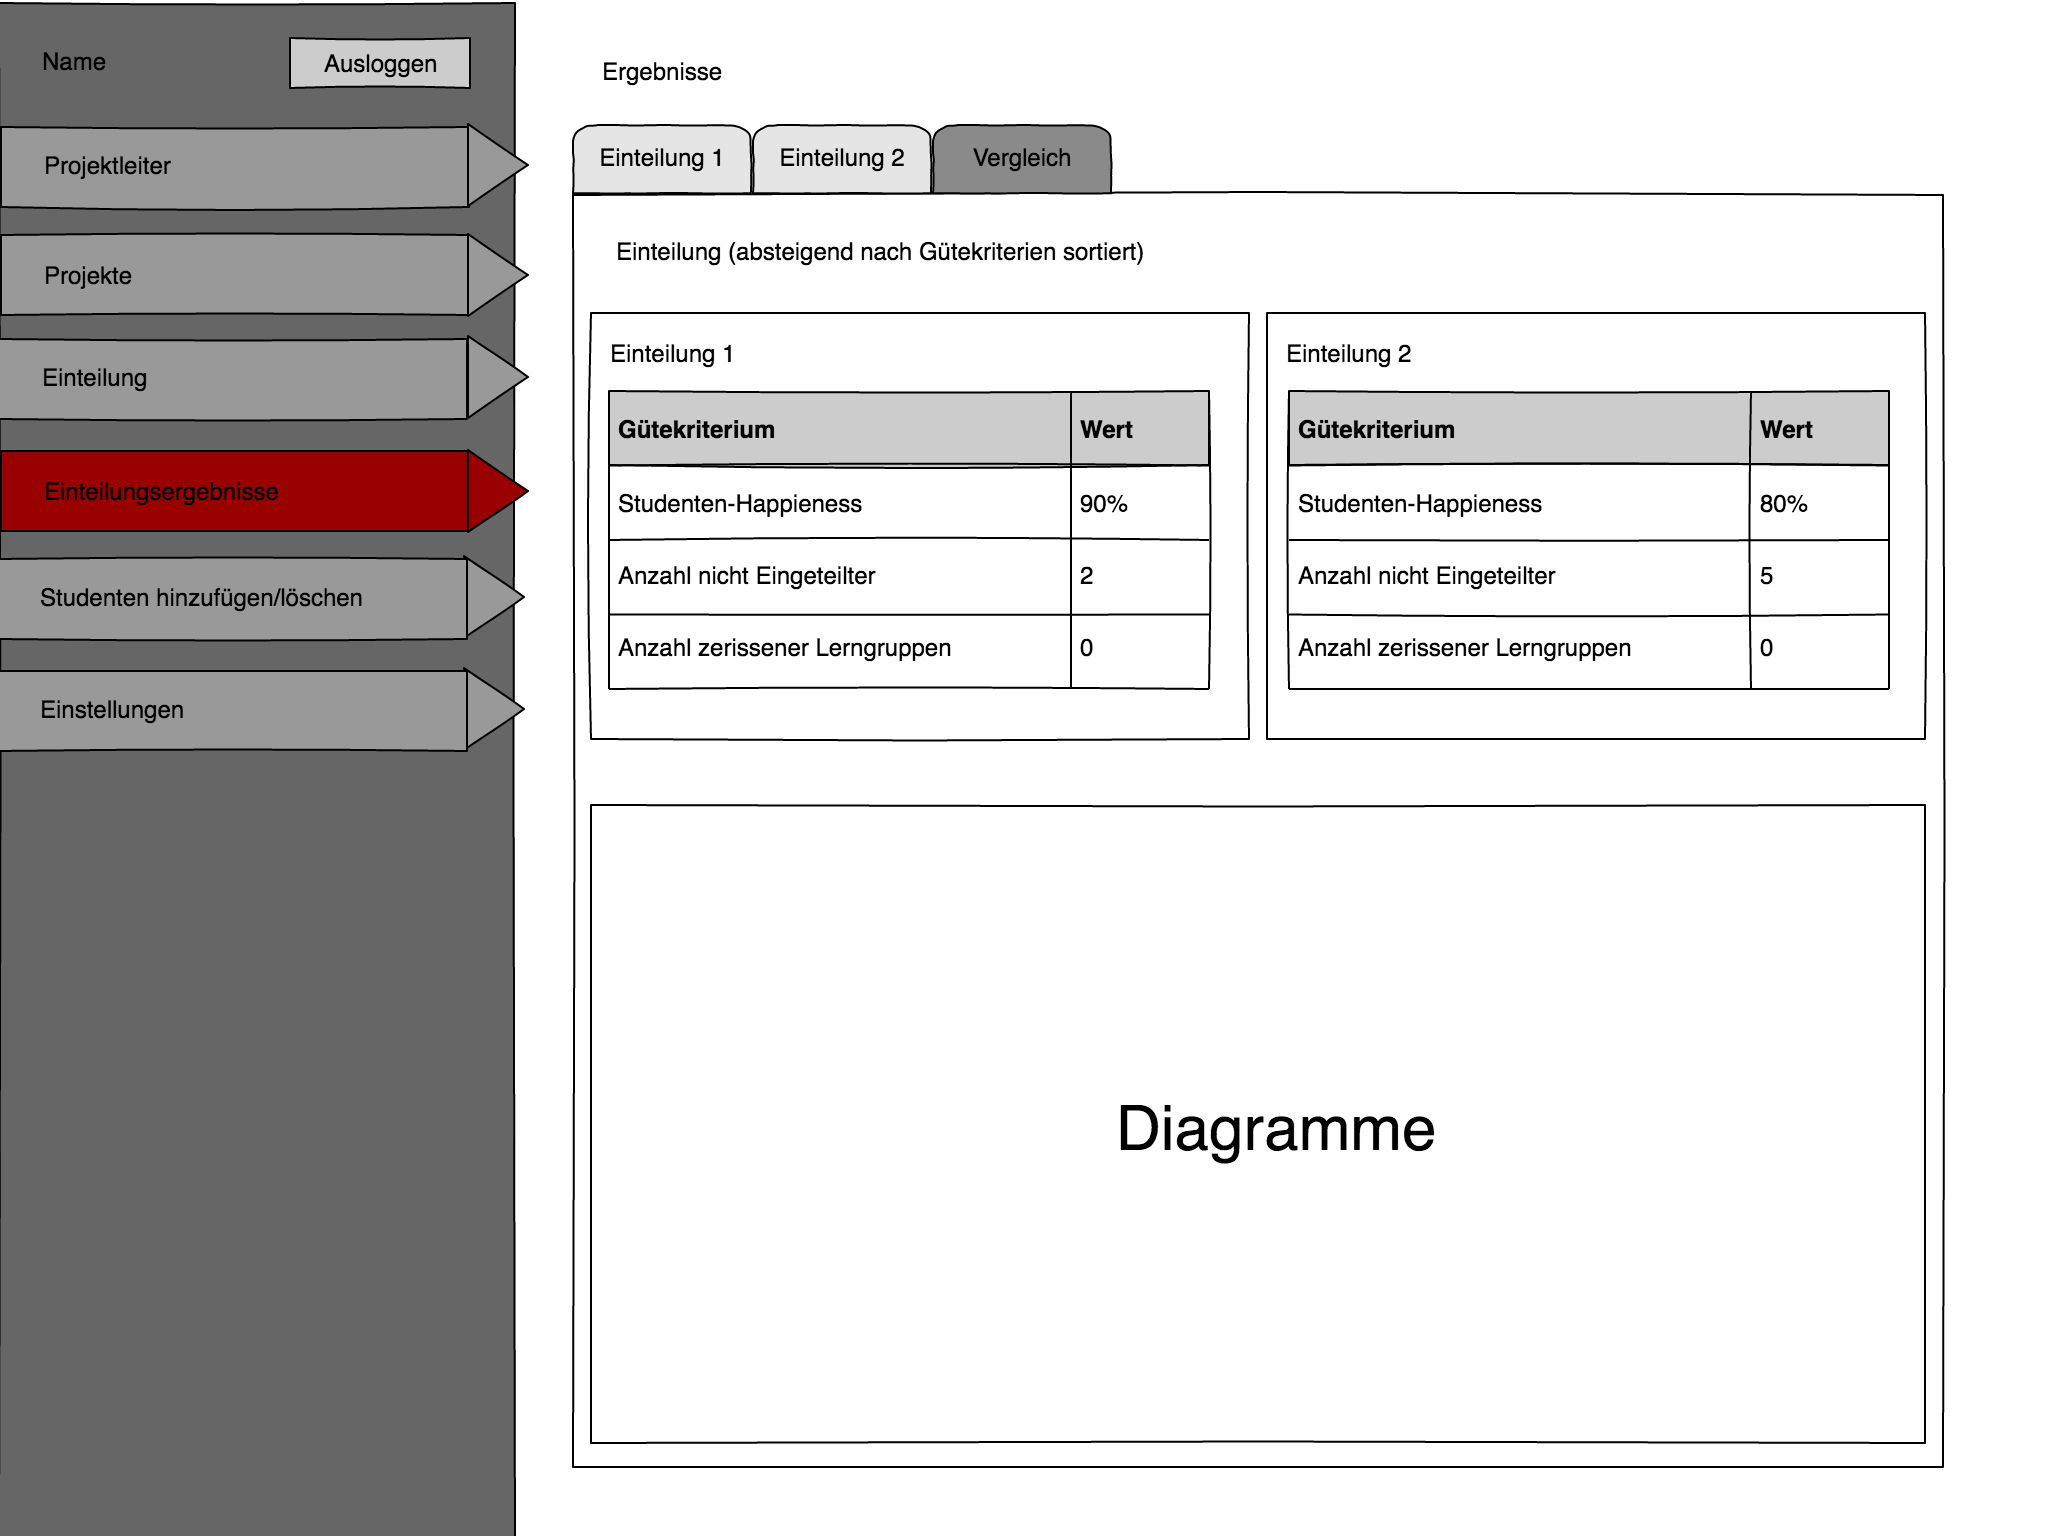
\includegraphics[width=\textwidth,
keepaspectratio=true]{gui/adminergebnissevergl.png}}
\captionof{figure}{Vergleichsansicht} \label{GUIvergleich}
\medskip
\fbox{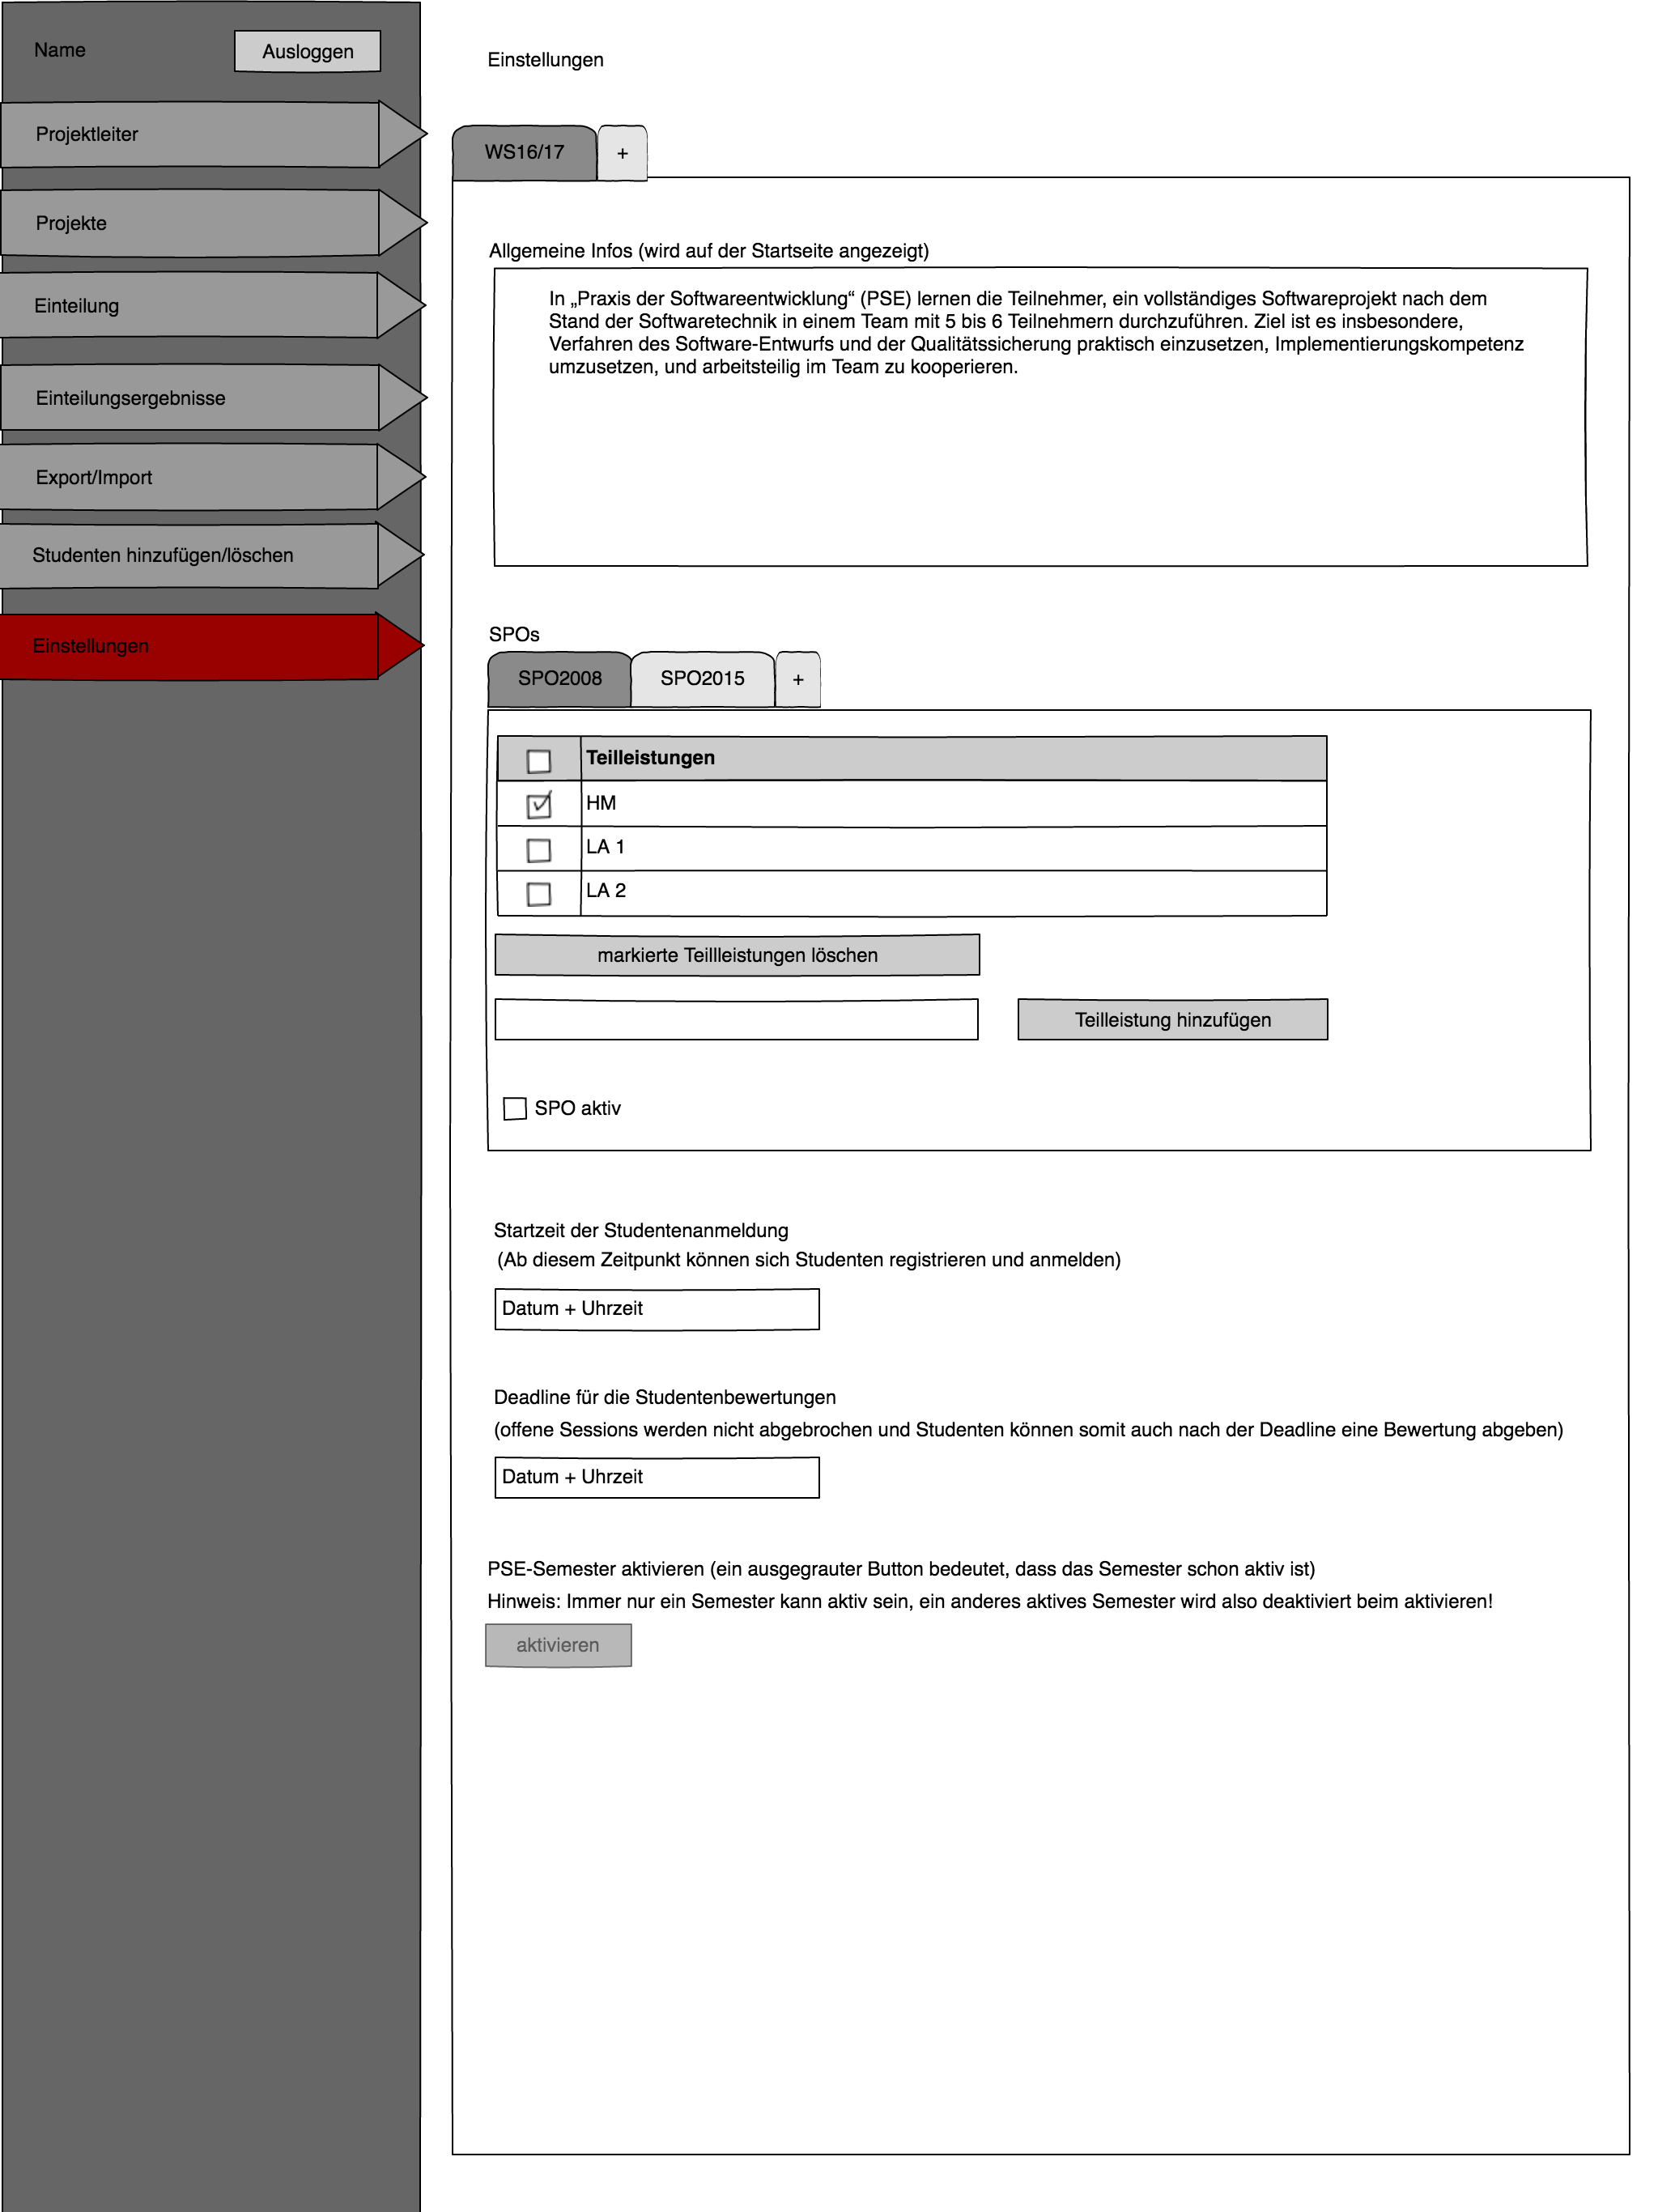
\includegraphics[width=\textwidth,
keepaspectratio=true]{gui/adminproperties.png}}
\captionof{figure}{Einstellungen} \label{testBild}
\medskip
\fbox{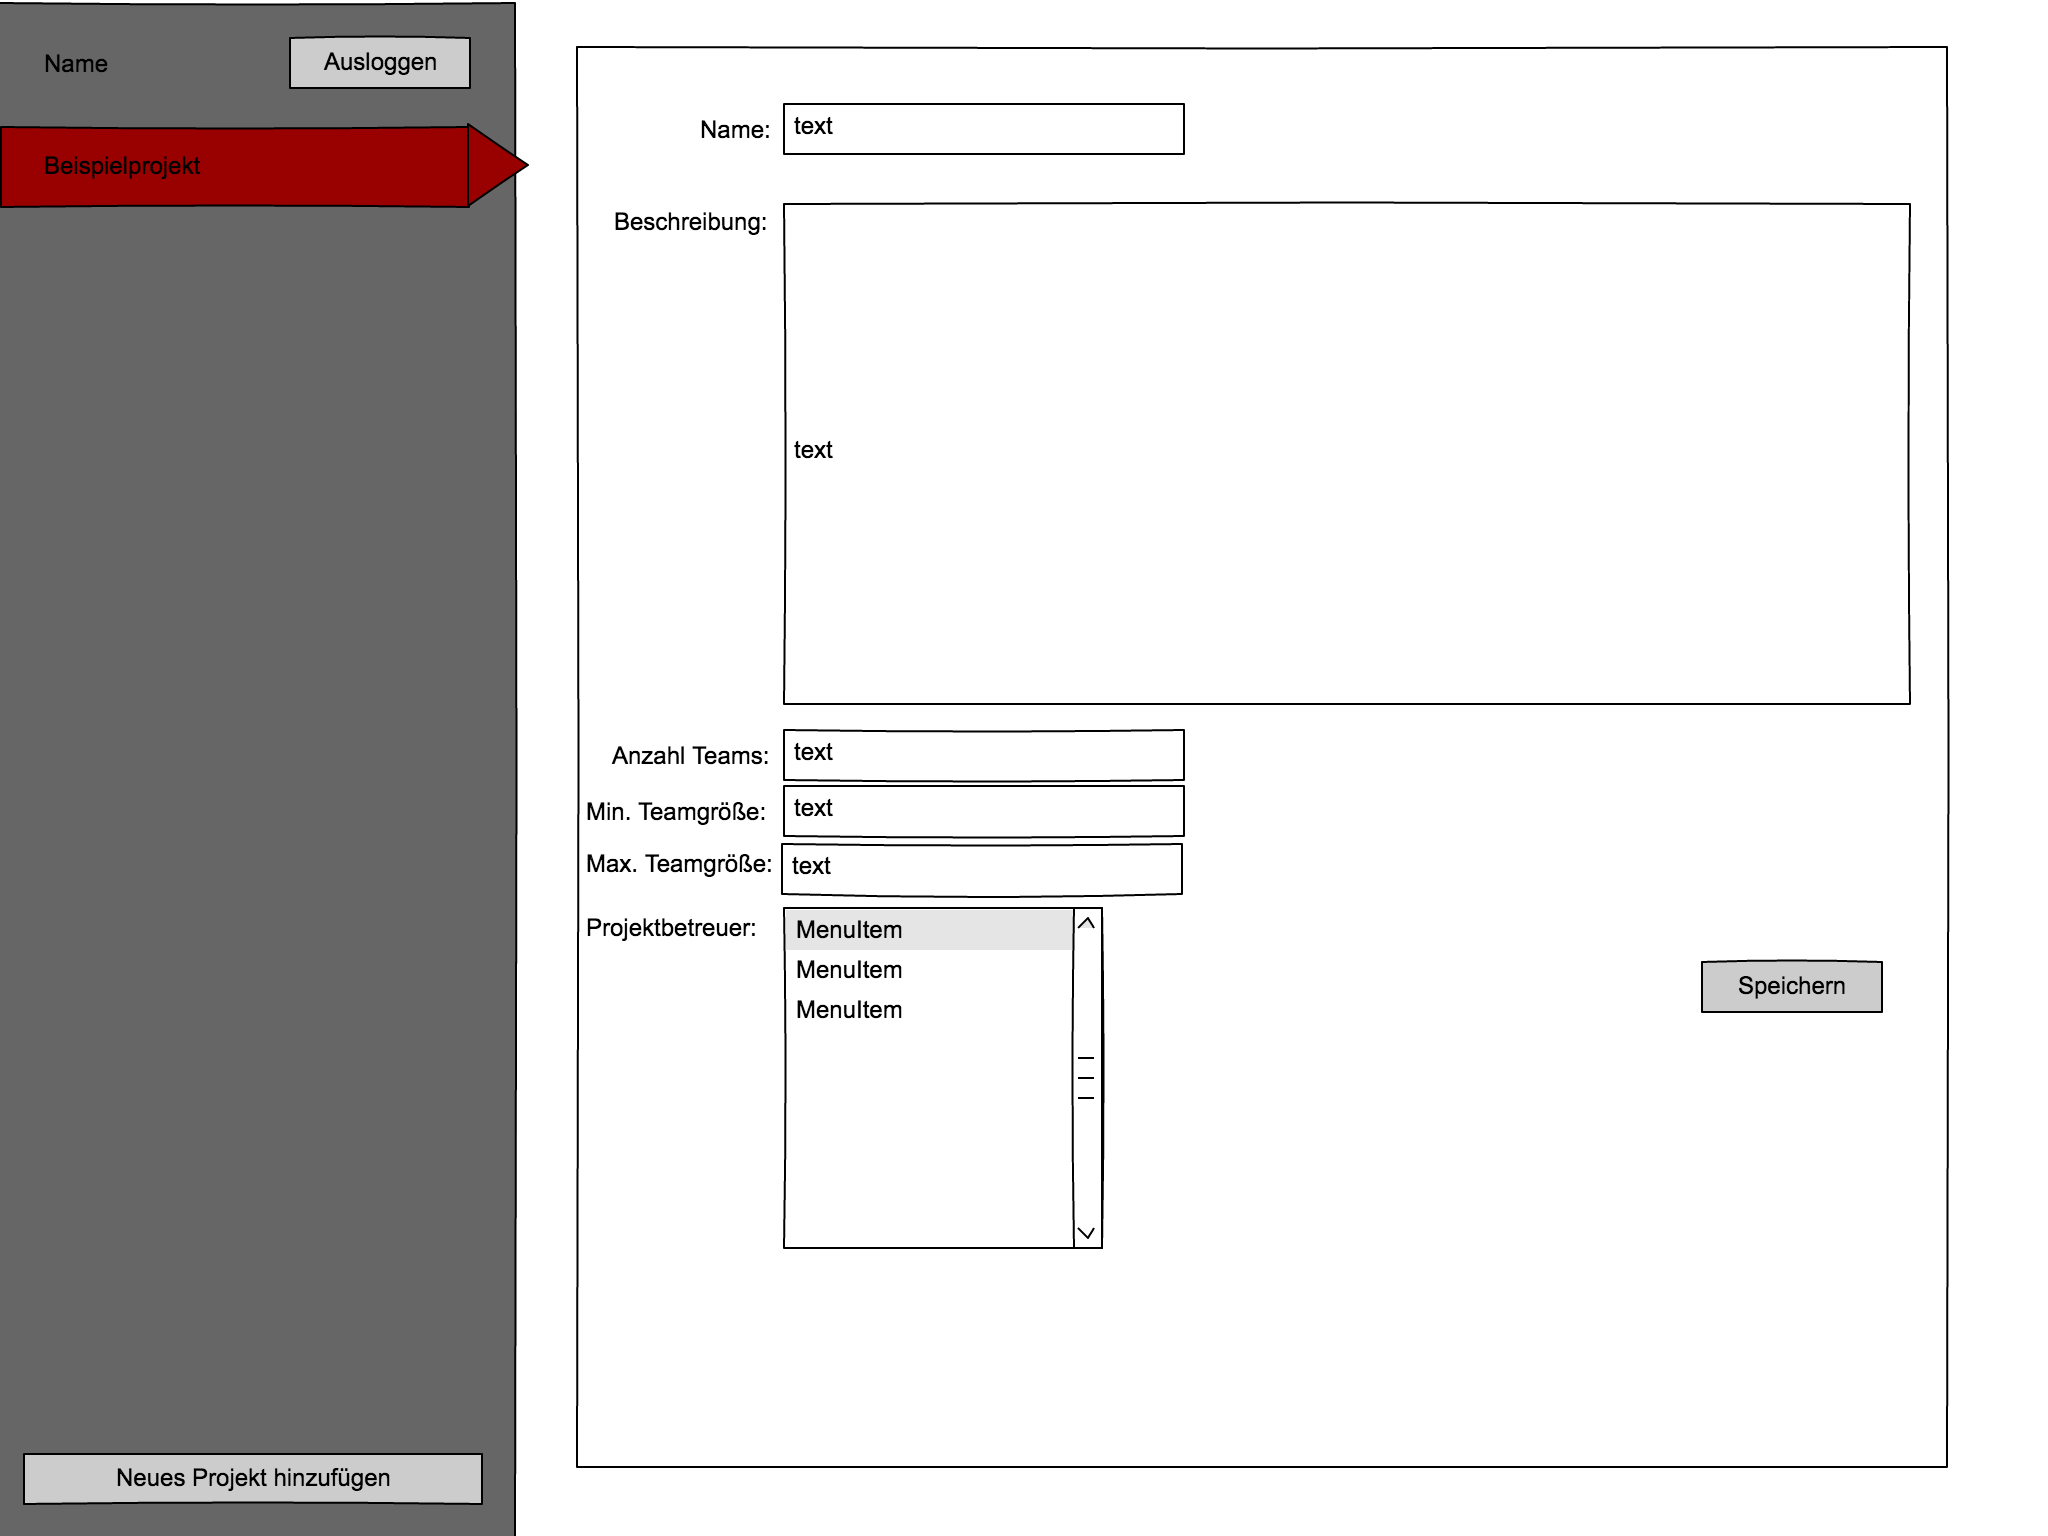
\includegraphics[width=\textwidth,
keepaspectratio=true]{gui/projleiterprojekte.png}}
\captionof{figure}{Betreueransicht} \label{GUIeinstellung}
\medskip
}
%TODO LIZENZ
\end{enumerate}
\pagebreak
\printglossaries
\end{document}
